% !TEX TS-program = pdflatex
% !TEX encoding = UTF-8 Unicode

% This is a simple template for a LaTeX document using the "article" class.
% See "book", "report", "letter" for other types of document.

\documentclass[11pt]{article} % use larger type; default would be 10pt

\usepackage[utf8]{inputenc} % set input encoding (not needed with XeLaTeX)
\usepackage[english]{babel}
\usepackage{hyperref}
%\usepackage[cp1250]{inputenc}
%\usepackage[utf8]{inputenc}
\usepackage{latexsym}
\usepackage{amsfonts}
\usepackage{times}
\usepackage{xcolor}
\usepackage{graphicx}
\usepackage{crayola}
%\usepackage{datum}
\usepackage{xspace}
\usepackage{algorithmicx}
\usepackage{natbib}
\usepackage{authblk}
\usepackage{longtable}
\usepackage{rotating}
\usepackage{pdflscape}


\renewcommand{\textfraction}{.05}
\renewcommand{\topfraction}{.95}

\oddsidemargin 5pt \evensidemargin 5pt \marginparwidth 20pt
\marginparsep 10pt \topmargin -12 true mm \headheight 12pt \headsep 25pt
\textheight 23 true cm \textwidth 16 true cm
\columnsep 10pt \columnseprule 0pt

% title page --------------------------------------------------------------

\newcommand*{\affaddr}[1]{#1} % No op here. Customize it for different styles.
\newcommand*{\affmark}[1][*]{\textsuperscript{#1}}
\newcommand*{\email}[1]{\texttt{#1}}

\title{\LARGE\textbf{Social Network Analysis:}\protect\\ Bibliographic Network Analysis of the Field and its Evolution\\ Part 2. Analysis of Co-occurence Networks}
%\thanks{\textcolor{BrickRed}{\textbf{Applied Statistics}}, Ribno, 23-26. September 2018}

\author{%
Daria Maltseva\affmark[1], Vladimir Batagelj\affmark[1,2,3]\\
\affaddr{\affmark[1]NRU HSE Moscow}\\
\affaddr{\affmark[2]IMFM Ljubljana}\\
\affaddr{\affmark[3]IAM UP Koper}\\ \email{d\_malceva@mail.ru}\\
\email{vladimir.batagelj@fmf.uni-lj.si} %\\
%\affaddr{\LaTeX\ University}%
}
% \author{Darja Maljceva, Vladimir Batagelj  IMFM Ljubljana, IAM UP Koper, NRU HSE Moscow}


% user's macros ----------------------------------------------------------
\newcommand{\Pajek}{\texttt{\textbf{Pajek}}\xspace}
\newcommand{\WoSPajek}{\texttt{\textbf{WoS2Pajek}}\xspace}
%\newcommand{\Pajek}{Pajek}
\newcommand{\keyw}[1]{\textcolor{red}{\emph{#1}}}

\newcommand{\WA}{\mathbf{W\!\!A}}
\newcommand{\AW}{\mathbf{A\!\!W}}
\newcommand{\WK}{\mathbf{W\!K}}
\newcommand{\KW}{\mathbf{K\!W}}
\newcommand{\WC}{\mathbf{W\!C}}
\newcommand{\WJ}{\mathbf{W\!J}}
\newcommand{\Ci}{\mathbf{Cite}}
\newcommand{\Co}{\mathbf{Co}}
\newcommand{\Cn}{\mathbf{Cn}}
\newcommand{\Ct}{\mathbf{Ct}}
\newcommand{\N}{\mathbf{N}}
\newcommand{\NP}{N\!P}
%\newcommand{\diag}{\operatorname{diag}}
\newcommand{\sgn}{\operatorname{sgn}}
% \newcommand{\WA}{\mathbf{W\!A}}

\newcommand{\important}[1]{\textcolor{NavyBlue}{#1}}
\newcommand{\RR}{\Bbb{R}}
\newcommand{\NN}{\Bbb{N}}
\newcommand{\ZZ}{\Bbb{Z}}
\newcommand{\QQ}{\Bbb{Q}}
\newcommand{\network}[1]{\mathcal{#1}}
\newcommand{\vertices}[1]{\mathcal{#1}}
\newcommand{\edges}[1]{\mathcal{#1}}
\newcommand{\arcs}[1]{\mathcal{#1}}
\newcommand{\Net}{\network{N}}
\newcommand{\argmin}{\mathop{\mbox{argmin}}\nolimits}
\newcommand{\relation}[1]{\textbf{\emph{$\_\!\_$~#1~$\_\!\_$\,}}}
\newcommand{\functions}[1]{\mathcal{#1}}
\newcommand{\define}[1]{\emph{\textcolor{red}{#1}}}
\newcommand{\card}[1]{\mbox{card}(#1)}
\newcommand{\URL}[1]{{\footnotesize\texttt{#1}}}
\newcommand{\tita}[1]{\textit{#1}}      % italic
\newcommand{\cling}{\mathbf{C}}
\newcommand{\unitX}{\mbox{X}}
\newcommand{\unitY}{\mbox{Y}}
\newcommand{\unitZ}{\mbox{Z}}
\newcommand{\outdeg}{\mbox{outdeg}}
\newcommand{\indeg}{\mbox{indeg}}
\newcommand{\ato}{\mathrel{:=}}
\newcommand{\unit}{\mbox{X}}
\newcommand{\Units}{\vertices{U}}
\def\Min{\mathop{\mbox{Min}}\nolimits}
\def\Max{\mathop{\mbox{Max}}\nolimits}
\newcommand{\graph}[1]{\mathcal{#1}}
\newcommand{\function}[3]{#1\,{:}\ #2\to#3}
\newcommand{\Gph}{\network{G}}
\newcommand{\GphH}{\network{H}}
\newcommand{\Graph}{\mathbf{G}}
\newcommand{\tit}[1]{\textit{#1}}      % italic
\newcommand{\diag}{\mbox{diag}}
\newcommand{\func}[1]{\textit{#1}}
\newcommand{\Relation}[1]{\mathbf{#1}}
\newcommand{\Time}{\mathcal{T}}
%\newcommand{\cmdkey}{\raisebox{-.035em}{\includegraphics[height=.75em]{command.pdf}}}
\newcommand{\cmdkey}{\raisebox{-.025em}{\includegraphics[height=.7em]{command.pdf}}}
\newcommand{\Mw}{\mathop{\raisebox{-1.5pt}{\mbox{$\Box$\kern-.55em\raisebox{2.5pt}{{\tiny $r$}}\kern2.9pt}}}}
\newcommand{\Mv}{\mathop{\raisebox{-1.5pt}{\mbox{$\Box$\kern-.55em\raisebox{2.5pt}{{\tiny $h$}}\kern2.9pt}}}}

\newcommand{\Remark}[1]{\ifodd\value{page} \normalmarginpar
 \else \reversemarginpar \fi \marginpar{{\footnotesize #1}} }

\newcommand{\clock}{\count254=\time \divide\count254 by 60
 \count255=\count254 \multiply\count255 by -60
 \advance\count255 by \time
 \ifnum\count254<10 0\fi\number\count254\,:\,%
 \ifnum\count255<10 0\fi\number\count255}

 \renewcommand{\textfraction}{.05}
 \renewcommand{\topfraction}{.95}

\oddsidemargin 5pt \evensidemargin 5pt \marginparwidth 60pt
\marginparsep 10pt \topmargin -12 true mm \headheight 12pt \headsep 25pt
\textheight 23 true cm \textwidth 16 true cm
\columnsep 10pt \columnseprule 0pt

\newcommand{\denseFont}{\fontencoding{T1}\fontfamily{phv}\fontseries{mc}\fontshape{n}\fontsize{10}{11pt}\selectfont}


%\newcommand{\diag}{\mathop{\rm diag}\nolimits}

%\graphicspath{{./pics/}}
\graphicspath{{./pics/}}

%******************************************************************************
\begin{document}


\hypersetup{pdfauthor={D. Maltseva, V. Batagelj}}
%\hypersetup{pdftitle={Bikes; 1. data}}
\hypersetup{pdftitle={SNA. The evolution of the field}}

\maketitle

\begin{abstract}
Abstract ...
\\[4pt]
\textbf{Keywords:}  social network analysis, bibliographic networks, main path,  island,
\end{abstract}


%******************************************************************************

\section{Introduction}

This paper presents the second part of the results of the study on the development of social network analysis (SNA) discipline and its evolution over time. We aim to implement comprehensive approach for the identification of the current trends of the Social network analysis field development -- in terms of the representation of various disciplinary areas, groups of scientists, and thematic agenda in the field. The provided methodology of \textbf{bibliometric networks analysis} already proved to be productive in a set of studies of different scientific fields and topics \citep{kejzar,Understand,PeerRew}.It allows allocating key publications and actors (authors, research groups, institutions, journals) in the SNA field, main topics and scientific ideas, connections between them and their evolution through time, as well as analyzing networks of co-authorship, co-occurence, citation and co-citation between different bibliographic entities. \medskip 

The development of the SNA field was reflected in a set of studies focused both on its historiographical description \citep{SNAdev} and bibliometric analysis of publications and journals involved to the field (including \textit {Social Networks}). Different authors studied citation structures of works and journals \citep{normSci,leydes,Understand}, collaboration structures in sense of co-authorship \citep{SNAinf, leydes,Understand}, structures of co-citations between works, authors, and journals \citep{brandes}, topical structures and keyword co-occurence networks \citep{leydes,lookingglass}. Attention was also given to different subfields (subtopics)  \citep{central,kejzar,Understand,batagelj2019} and subdisciplines within the field \citep{SNAinf,borgatti,lazer,varga}. We presented the comrehensive review of these studies in the first paper [first paper citation]. 

Our dataset consists of articles from the \textit{Web of Science} Clarivate Analytics database (Core Collection) and those published in the main journals in the field, created by searching for the key word “social network*.”  Using \textbf{WoS2Pajek 1.5} \citep{wos2pajek}, we transformed our data into a collection of networks: one-mode citation network \textbf{Cite} on works (from the field CR of WoS file description) and two-mode networks -- the authorship network $\WA$ on works $\times$ authors  (from the field AU),  the journalship network $\WJ$ on  works $\times$ journals  (from the field CR or J9), and the keywordship network $\WK$ on works  $\times$ keywords (from the fields ID, DE or TI). An important property of all these networks is that they share the same first node set -- i.e. the set of works (papers, reports, books, etc.) -- wich means that they are \keyw{linked} and can be easily combined using the network multiplication into new \keyw{derived}  networks \citep{Understand}. Works that appear in descriptions can be of two types: those which have full descriptions (\textit{hits}), and those which were only cited (listed in the CR fields, but not contained in the hits).  the cited only  works  $(DC=0)$ only partial descriptions are provided: we have information only about the \textit{first} author, the journal and the publication year, and we have no information on the keywords (as there are no titles in ISI names and cited works). That is why for further analysis we constructed networks, which contain only works with complete description $(DC>0)$. We labeled these \keyw{reduced networks} \textbf{CiteR}, \textbf{WAr}, \textbf{WJr}, and \textbf{WKr}. In obtained networks, the sizes of sets are as follows: works $|W| = 70,792$, authors $|A| = 93,011$, journals $|J| = 8,943$, key words $|K| = 32,409$. The procedure of data collection, cleaning and networks construction is presented in detail in the first paper [citation].\medskip 

In the first paper, we presented the analysis of basic networks \textbf{Cite}, \textbf{WA}, \textbf{WK}, and \textbf{WJ} (and their reduced versions), and thus extracted the  most cited works, authors and journals with the largest amount of works, and most often used keywords in the SNA field. Using the Search path count approach, we extracted the main path, key-route paths and link islands in the citation network \textbf{Cite}. Based on the probabilistic flow node values, we identified the most important articles. The results show that starting from its institutionalization in the 1980-1990's, SNA field has grown significantly in terms of the number of publications and the amount of disciplines involved into the research using SNA approach. The number of publications shows the constant growth, and on average it doubles every 3 years. The analysis confirmed the previous studies on the SNA field development using citation network analysis. Up to the middle of 1990's the most ``important'' works belong to the authors from the \textit{social sciences}, and starting from 2000's the field experience the ``invasion of physicists''. To our surprise, from 2010's both groups experience the ``invasion'' of scientists from a completely another field -- \textit{animal SNA}. According to the analysis of journals, another active field of SNA research goes from the \textit{Computer science} field.  \medskip 

The obtained results put new question to the research. From one side, the lists of most cited works, most used journals and, especially, keywords (with top words \textit{social, network} and \textit{analysis}) do not contradict our basic knowledge of the SNA field, and thats why a conclusion on the relevance of the obtained data to the research objects can be done. From another side, the citation network analysis was not able to detect some well known topic groups from the field of social science, who has been very active recently, such as \textit{probabilistic approach} with Snijders and Robins as representatives, \textit{signed networks} developed by Doreian, etc. The explanation of this situation may lie in the nature of the \textbf{Cite} citation network and algorithms of \textbf{Main path} and \textbf{Islands} used for identification of main subgroups from it.\medskip 

That's why in the current paper we answer to the posed questions using more complex analysis of other available networks, derieved from the basic networks with the procedures of \textbf{networks multiplication} and using \textbf{fractional approach} for normalization. In the following parts, we provide the description of the \textit{topic structure of the field} based on the keywords co-occurence netwok analysis, the structures of \textit{authors collaboration} and keywords associated with coathorship islands, patterns of \textit{citation and co-citation} among authors and journals.\medskip 


%******************************************************************************

\section{Data}

\subsection{Derieved networks}

Using basic networks \textbf{CiteN}, \textbf{WAn}, \textbf{WJn}, \textbf{WKn} and their reduced versions \textbf{CiteR}, \textbf{WAr}, \textbf{WJr}, \textbf{WKr} we constructed other networks for the further analysis using the procedure of \textbf{networks multiplication}. Two-mode networks are composed of descrete two-mode arrays, which can be combined using matrix multiplication. The product of two compatible networks is the network corresponding to the product of matrices corresponding to the given networks. Two two-mode networks are \textit{compatible} for multiplication, if the second set of vertices in the first network is equal to the first set of vertices in the second network. If all weights in two two-mode networks are equal to 1, then the product of the weights multiplication will also be equal to 1.\citep{OnBibl,Understand}. \medskip 

In our case, this shared set is a set of works (papers, reports, books, etc.), which \keyw{links} different basic and reduced networks to each other. Using multiplication, we constructed \keyw{derieved networks} of two types. First type are one-mode networks made by the multiplication of two two-mode networks. Multiplying \textit{same} two-mode networks, we got the network of keywords co-occurence \textbf{KK} (\textbf{WK}T * \textbf{WK}) and collaboration network \textbf{AA} (\textbf{WA}T * \textbf{WA}). The weight of link between two nodes \textit{w(k1,k2)} in keywords co-occurence \textbf{KK} network shows how many times the keywords \textit{k1} and \textit{k2} were used together in the same work. The wight of edge between two authors \textit{w(u,v)} in collaboration network \textbf{AA} shows the number of works to which \textit{u} and \textit{v} both contributed. Multiplying \textit{different} two-mode networks (which still share the same set of nodes), we constructed the network of authors and keywods \textbf{AK} (\textbf{WA}T and \textbf{WK}) counting in how many works the author \textit{u} used the keyword \textit{k}. \medskip 

Another type of networks are those which are produced by three steps of multiplication, when we use some network, such as citation network, for a ``projection'' of relations between other bibliographic entities. Multiplying \textbf{WA} networks through the \textbf{Cite} network, we got the network of citations among authors \textbf{CiteA}, where the weight of edge between two authors \textit{w(u,v)} shows the number of times when author \textit{u} cited author \textit{v}. Multiplying \textbf{WJ} networks through the \textbf{Cite} network we constructed the network of citations among journals \textbf{CiteJ}, where the weight of edge between two journals \textit{w(i,j)} shows the number of times when journal \textit{i} cited journal \textit{j}. Similarly, out of \textbf{WA}, \textbf{WJ} and \textbf{Cite} networks we constructed the networks of co-citations among authors \textbf{ACoj} and and journals \textbf{JCoj}, where the weight of edge between two nodes (authors or journals) shows the similarity of their citation patterns.\medskip 

The detailed description on each derieved network construction is presented in the corresponding sections. \medskip 

\subsection{Normalized networks} 

It was shown that the multiplication has some limitations, such as the overrating of the contribution of bibliographic entities with many ties (works having a lot of authors or keywords, journals having a lot of works). That`s why the \textbf{fractional approach} (Gauffriau et al. 2007, \cite{OnBibl}) was proposed, which takes into account the contribution of bibliographic entities (works, authors, or journals), normalizing the weights between them in such a way their input is equal to 1. \medskip 

Let us provide the example of authorship two-mode network \textbf{WA}. In regular network, the outdegree is equal to the number of authors of this work, and the indegree is equal to the number of works to which author contributed. The normalization create network $n(\textbf{WA})$ where the weight of each arc is divided by the sum of weights of all arcs having the same initial node as this arc (outdegree or outsum of a node). A contribution of each paper p was equal to 1, and we assume that each author contributed to the work equally. \smallskip 

\[ n(\mathbf{WA})[w,a] = \frac {\mathbf{WA}[w,a]}{\max(1,\textrm{outdeg}(w))}\] \medskip 

A similar normalization of collaboration links, but with \textit{outdegree(w) -- 1} instead of \textit{outdegree(w)} was proposed by Newman (2001), who interpreted the weight of link between two authors as a proportion of time spent for the collaboration with each co-author (that's why ``collaboration'' with herself or himself is not taken into account). \medskip 

The proposed ways of normalization can be used in other two-mode networks. The detailed description of their usage for networks creation is presented in the corresponding sections. 

%******************************************************************************
\section{Keywords co-occurence: Topic structure of the field}  

\subsection{Network KKn production}

To construct the one-mode network \textbf{KKn}, we normalized the reduced \textbf{WKr} network in such a way that all works have equal contribution by keywords they provide: the fractional contribution of each complete subgruph in $KKn$ is equal to 1. With this normalization, the works with large number of keywords are not overrepresented -- the inputs of works having 1 and 10 keywords are the same. Normalization creates network $n(WKr)$ where the weight of each arc [w, k] is divided by the sum of weights of all arcs having the same initial node (works) as this arc (outdegree of a node). The normalized network $WKn$ was transposed and multiplied with itself. In the obtained network, the loops were deleted and bidirected arcts were transformed to edges (with summation of the line weights). The obtained network KKn consists of 32,409 nodes and 2,799,530 edges. In the obtained network, the weight of the edges between the nodes (keywords) is equal to the \textit{fractional} co-occurence of keywords $i$ and $j$ in the same works.\medskip

\[ \mathbf{KKn} = n(\mathbf{WK})^T * n(\mathbf{WK}) \]
where 
\[ n(\mathbf{WK})[w,k] = \frac {\mathbf{WK}[w,k]}{\textrm{max}(1,\textrm{outdeg}(w))}\]
\medskip

\subsection{Networks of key words co-occurence}

Exploratory analysis showed that in the obtained network the most frequentlty words \textit{social}, \textit{network}, and \textit{analysis} were connecting most of the other keywords, that`s why we excluded these 3 nodes from the network. Using Islands approach, we aimed to obtain subnetworks sized from 2 to 75 nodes. We got a large number of islands (342), where the majority of islands (301) represent just pairs of keywords. The main island includes 75 nodes; there are also some islands of smaller sizes. \medskip

Large part of the Main island (Figure~\ref{kkmain}) are the keywords on the topic of networking sites and social media (such as \textit{networking, media, online, site, facebook, internet, technology, web 2.0}). Other central nodes are \textit{information} associated with networking group,  words \textit{diffusion} and \textit{privacy}, as well as \textit{base} and \textit{datum} (which also have links to many other keywords, including \textit{big}, and \textit{mining}). Other two central keywords are \textit{model} and \textit{graph}, which are connected to each other and other nodes, such as \textit{dynamics, complex, spread, influence} (for the first one) and \textit{random, theory, centrality -- betweenness, large -- scale -- free, cluster} (for the second). These central nodes are also connected to the words \textit{community} and \textit{algorithm}, which have links to \textit{detection} and \textit{structure}. Other topics appeared in this subnetwork are associated with \textit{health} and \textit{education}. \medskip

\begin{figure}
\begin{center}
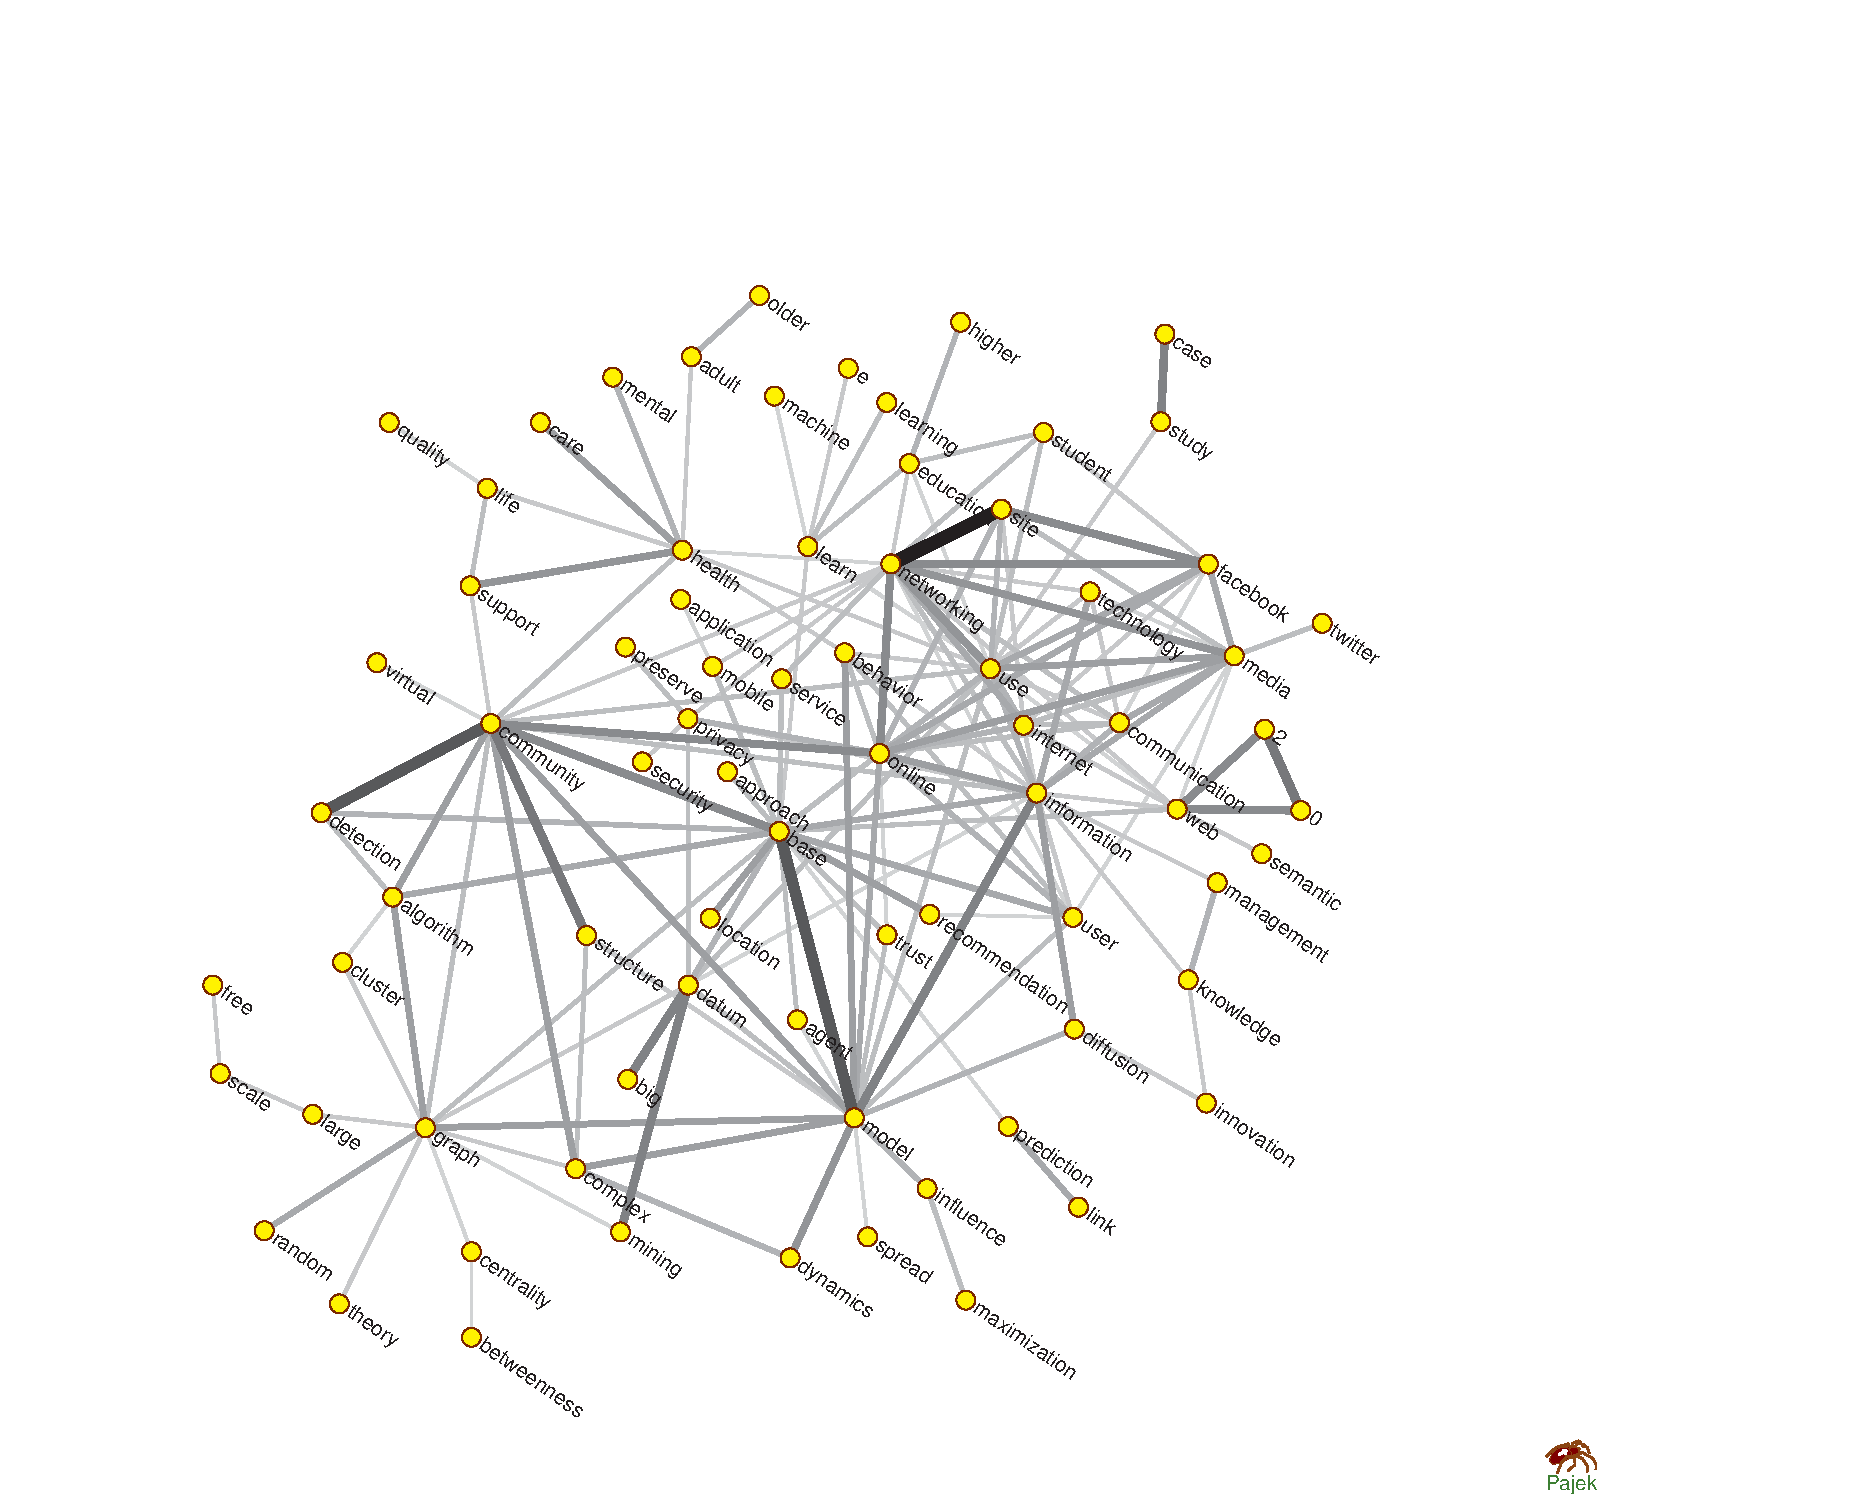
\includegraphics[width=\textwidth,viewport=93 35 665 585,clip=]{KKmain.pdf}
\end{center}
\caption{KK network Main Island} \label{kkmain}
\end{figure}

Other islands (largest are represented at the Figure~\ref{kkmid}\Remark{Probably, we do not need the Pic? Not much sense} identify some topics being studied in network analysis (\textit{strength, weak, tie; corporate - interlock - directorate; triadic - closure; small - world}, or some broad topics under study (\textit{organ - donor - donation; persecutory - delusion - paranoia; trade - international - migration}), as well as some stable phrases (\textit{special, issue, introduction}).\medskip


\begin{figure}
\begin{center}
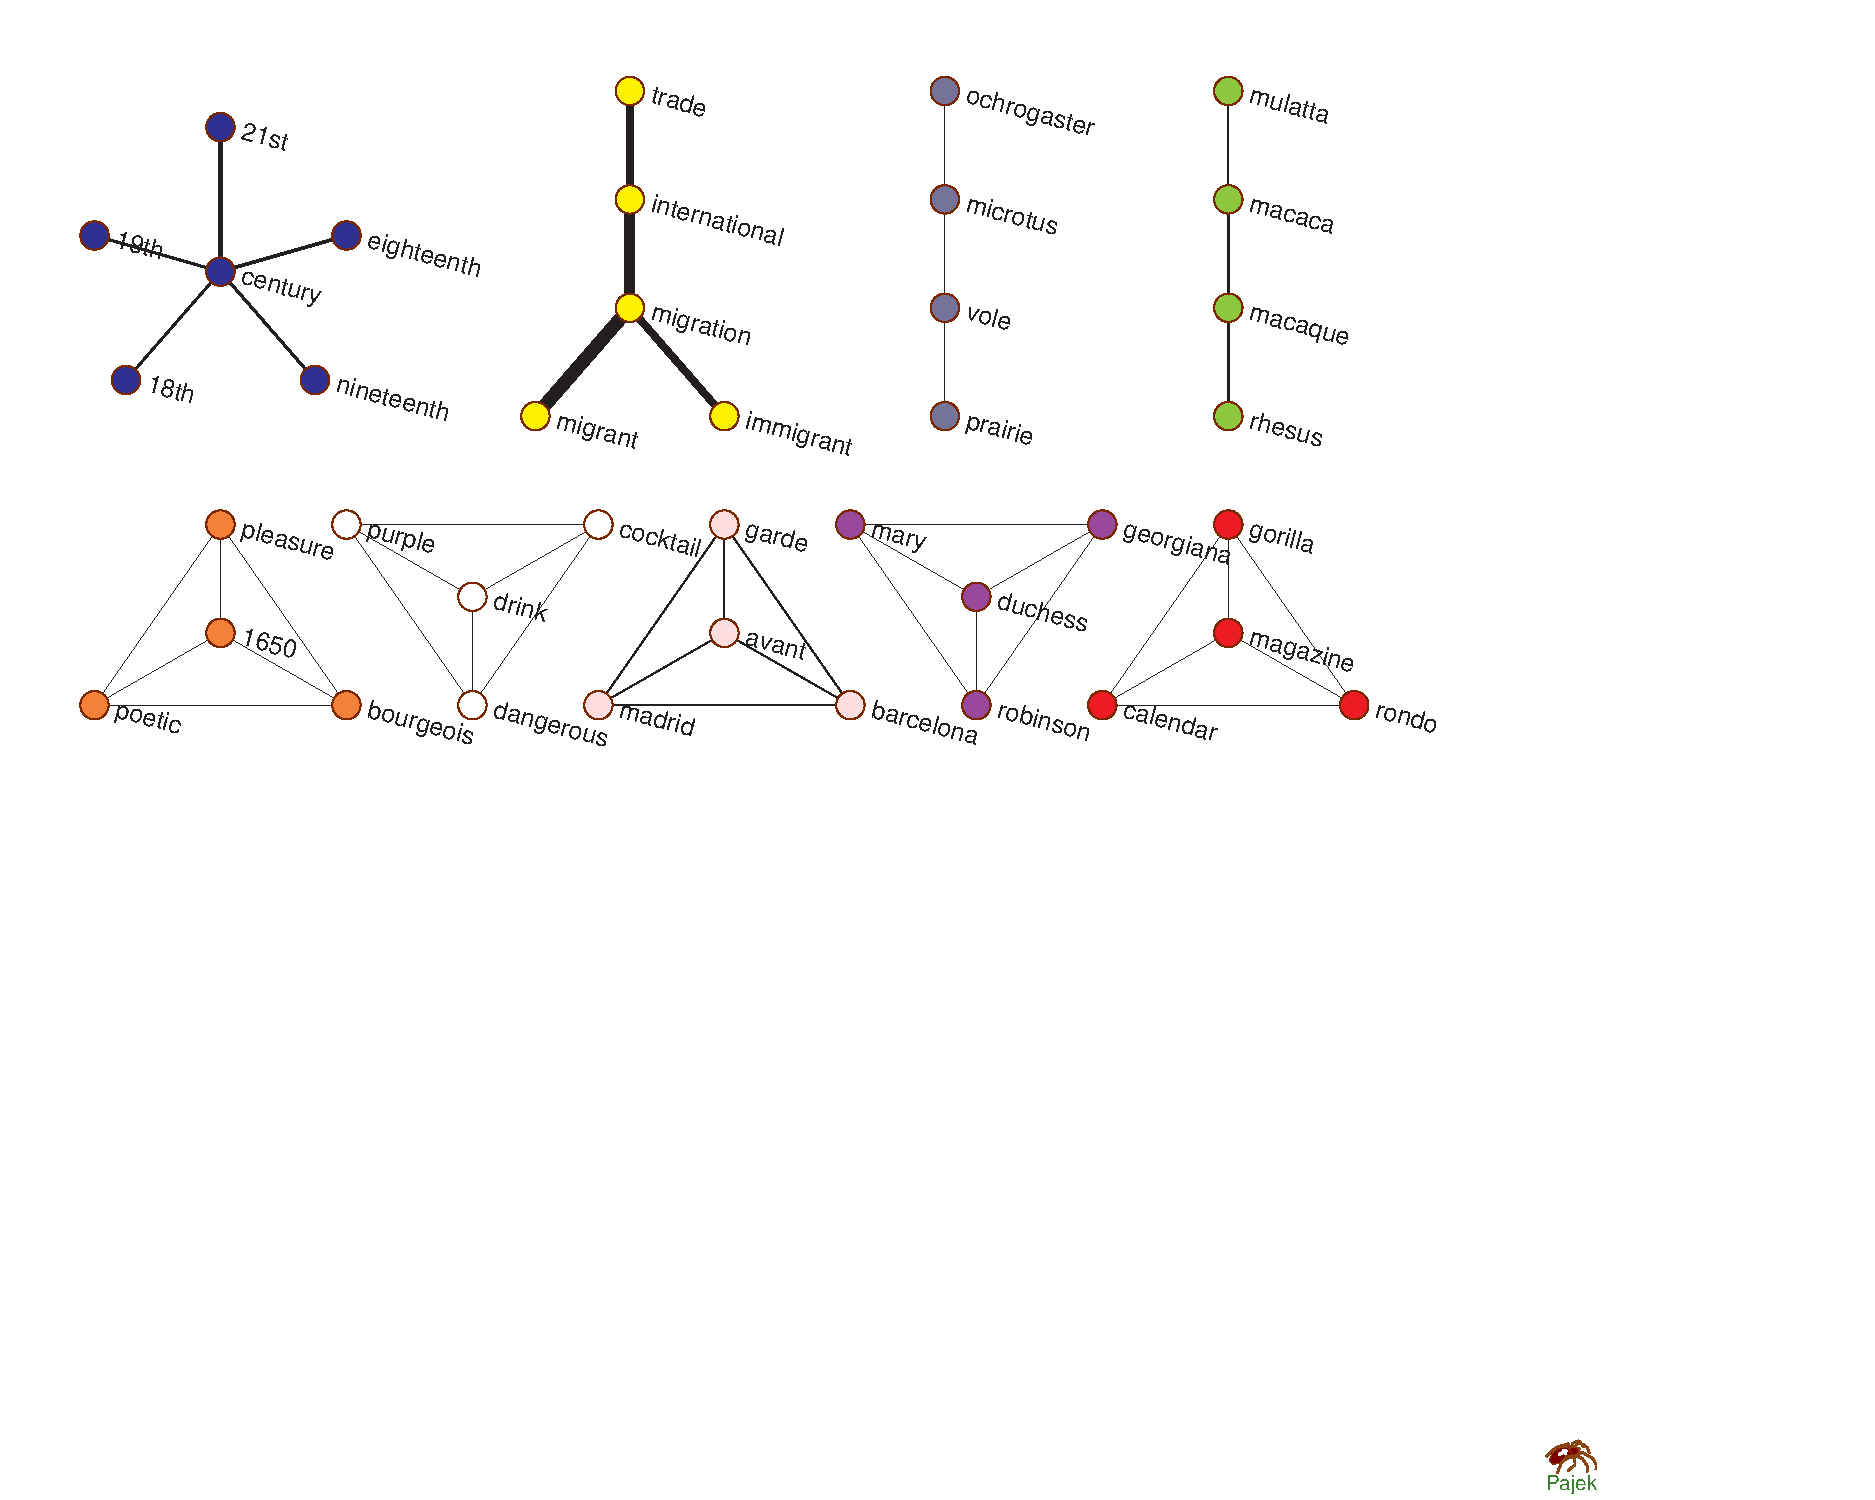
\includegraphics[width=\textwidth,viewport=35 356 695 686,clip=]{KKmid.pdf}
\end{center}
\caption{KK network Medium size Islands} \label{kkmid}
\end{figure}

%******************************************************************************
\section{Authors Collaboration}  

\subsection{Networks creation}  

There are different ways to create one-mode networks of collaboration between authors $AA$  out of two-mode networks of works and authors $WA$, which were presented and used in the previous studies \citep{OnBibl,Understand}. Multiplying the reduced \textbf{WAr} network, consisted of 70,792 works and 93,011 authors, to transposed WAr network, and using different types of normalizations, we created three collaboration networks \textbf{Co}, \textbf{Cn}, and \textbf{Ct'}. \medskip  

The standard and the easiest way to obtain the collaboration network is to create a \textbf{Collaboration network Co} \citep{OnBibl} by the multiplication of a transposed WAr network to original WAr network. In derived \textbf{Co} network, the weight of the edges between the nodes $i$ and $j$ is equal to total number of works author i and j wrote together. The loops in $Co$ are equal to the total number of works that each author have (which is also equal to the indegree values of the $WA$ network).  \medskip 

\[ \mathbf{Co} = \mathbf{WA}^T * \mathbf{WA} \] 

\textbf{Collaboration network Cn} uses \textbf{fractional approach}, where the contribution of authors to their own works and works written with co-authors is considered. The normalization creates network $n(WA)$ where the weight of each arc is divided by the sum of weights of all arcs having the same initial node as this arc (outdegree of a node). The network is constructed by the transposition of the $WA$ network and multiplying it with the (normalized) $n(WA)$ network.\smallskip

\[ n(\mathbf{WA})[w,a] = \frac {\mathbf{WA}[w,a]}{\max(1,\textrm{oudeg}[w])}\]
then 
\[ \mathbf{Cn} = \mathbf{WA}^T * n(\mathbf{WA}) \] 
\medskip
 
In the derived network Cn, the weight of the edges between the nodes (authors) is equal to the contribution of author $i$ to works, that he or she wrote together with author $j$ (which can be not symmetric). Then the \textbf{author's total contribution} to all his/her works is counted as a value of diagonal (loops) of a $Cn$ network for a certain author. Based on it, Batagelj and Cerinšek \citep{OnBibl} proposed \textbf{self-sufficiency index Si} as a proportion of author's contribution to all his/her works \textit{cnii} and her/his total number of works (which is equal to the value of Indegree of author in $WA$ network), and the \textbf{collaborativness index Ki}, which is complementary to it (is equal to 1 minus self-sufficiency). \medskip 

\[ \mathit{S_i} = \frac{\mathit{cn_{ii}}}{\textrm{indeg}_\mathbf{WA}(i)}\]

\[ \mathit{K_i} = \mathit{\textrm{1} - S_i} \]

Using another type of normalization -- Newman's normalization, who interprets collaboration in a “strict” way, as a collaboration only with others and not with author himself of herself, -- the \textbf{Collaboration network Ct'} was constructed.  In this case, for the initial $WA$ network the weight of each arc is divided by the sum of weights of all arcs having the same initial node as this arc (outdegree of a node) subtracting the initial author (which is 1). Then the network \textbf{Ct'} is constructed by the transposition of the regularly normalized $n(WA)$ network (used for \textbf{Cn} network production above) and multiplying it with the Newman normalized $n'(WA)$ network. \smallskip

\[ n'(\mathbf{WA})[w,a] = \frac{\mathbf{WA}[w,a]}{\max(1,\textrm{outdeg}(w)-1)}\]
then 
\[ \mathbf{Ct'} = n(\mathbf{WA})^T * n'(\mathbf{WA}) \] 

The obtained $Ct'$ is undirected without loops. The contribution of a complete subgraph corresponding to each work is 1. The weights of the edges between the nodes (authors) are equal to the total contribution of “strict collaboration” of authors i and j to works they wrote together. The total contribution for an author is counted by line weights -- it is equal to the sum of the weights of all the works he or she co-authored.  \medskip 

\subsection{Collaboration between authors}  

It was already shown in the first paper that the authors having the largest number of papers have Chinese and Korean names. The issue of the super-productivity of these groups of authors was discussed by \cite{harzing2015} -- this is the well-known \href{https://en.wikipedia.org/wiki/List_of_common_Chinese_surnames}{"three Zhang, four Li"} effect: 80\% of people in China have one of only around 100 surnames. Thus, there is a high chance that different authors, having the same surname and first letter of the name, shrink together, creating `multiple personalities'. This problem could be overcame if we would use a special ID (such as ORCID) for each scientist (but this information is not provided in WoS yet).  \medskip 

In this sense, it is not productive to look at the `most writing' authors. However, from the \textbf{Co} network we still get an important information about collaboration between groups of authors in terms of amount of works written by two authors together. In the obtained \textbf{Co} network, we made a link cut  at the level of at least 10 works written together, and got a subnetwork of 420 nodes, which includes 1 component of 58 nodes, 1 component of 9 nodes, 2 components of 7 nodes, 4 components of 6 nodes, 4 components of 5 nodes, 9 components of 4 nodes, and 23 components of 3 nodes. Almost half of the nodes (45\%) belong to the 95 components of the size 2. There are not so many authors who has 10 works written in collaboration, and even for those who have it is quite common to have them written in pairs. \medskip 

However, there are some extra cases. The component of 58 nodes is formed by the authors with Chinese and Korean names (Figure~\ref{CoMain}). Again, we can propose that this subgroup is a result of ``multiple personalities'': there still a higher chance that there are several (as an example) \texttt{ZHANG\_Z} collaborationg with several \texttt{LI\_Y}, whose names are merged together. The largest line weights are for \texttt{MA\_J} and \texttt{WANG\_Y}, who have 31 works written together. According to our database, the author with the name \texttt{Ma J.} has published works in different spheres such as computer science, social networks, energy, physics, or health. The second name of this author varies: it is \textit{Jing, Jun, Jiemin}, etc. Name \texttt{WANG\_Y} also varies: \textit{Wang YZ, Wang YC, Wang YW}, etc. Other such pairs with large amount of papers in common are \texttt{WANG\_B} and \texttt{WU\_B} (27), \texttt{GUO\_B} and \texttt{YU\_Z} (25). \medskip 

Several selected components of the size 3 and more are presented on Figure~\ref{CoSelected}. Some of these structures are complete subgroups, where everyone is connected to everyone: group of Khadilkar, Kantarcioglu, Thuraisingham, Khan, Abrol, Heaterly, working in the field of online social networks and social media (minimum 22 works written together); McCarty, Killworth, Bernard, Johnsen, and Shelley, working in the field of methods for measuring personal social networks (minimum 11 works written togeter, with 22 works between Killworth and Bernard); Kimura, Saito, Ohara, and Motoda, working in the field of artificial intelligence (minimum 23 works); Lax, Buccafurri, Nicolazzo, Nocera connected to Ursino, working in the field of online social networks (minimum 11 works); Kennedy, Green, Golinelli, Wenzel, Tucker connected to Zhou, working in the filed of family, sex, social support (minimum 10 works). Several groups represent more star-like structures: a group around Latkin with minimum 10 works with Mandell, and maximum 27 works with Davey-Rothwell, in the field of psychology and medicine; and a group around Kazienko, having maximum 28 works with Bródka analyzing complex networks. Other groups represent authors working in the field of medical studies (Vassilev, Rogers, Kennedy, end others), ERGM (group around Robins and Pattison, having 38 works written together), animal and human bahaviour (James, Croft, Krause, and Wilson; Farine, Sheldon, and Firth), rsik and desease social networks (Potterat; Muth, Rothenberg), blockmodeling (Batagelj, Ferligoj, and Doreian). Among 95 pairs, there are those with maximum values (number of works written in brackets): Fowler and Cristakis (43), Carminat and Ferrari (32), Borgatti and Everett (29), and well-known pairs such as Valente and Fujimoto (16), Maybody and Rezvania (15), Dunbar and Roberts (13), Barabasi and Posfai (11), Brandes and Lerner (11), Litwin and Stoeckel (10). \medskip 

\begin{figure}
\begin{center}
\includegraphics[width=0.8\textwidth]{CoLineCutCluster1.pdf}
\end{center}
\caption{Co net: Main component} \label{CoMain}
\end{figure}

\begin{figure}
\begin{center}
\includegraphics[width=0.8\textwidth]{CoLineCutSelectedIslands.pdf}
\end{center}
\caption{Co net: Selected components} \label{CoSelected}
\end{figure}

It is interesting to compare the number of works that author has with the values of her or his contribution to these works and level of collaborativeness with others (Table~\ref{collab}). Because of the ``multiple personalities'' problem we had to exclude the names of the Chinese and Korean authors from the output. The names are ordered by authors' fractional total contribution to the field.The authors with the indexes of collaborativeness larger then 50\% are marked in boldface.\medskip  

In terms of \textbf{largest productivity}, the top rated authors are social scientist R. Burt, followed by phisician M. Newman, who have total contribution larger then 50. They are followed by P. Doreian, H. Park, and R. Dunbar, whose total contribution is larger then 40. Other authors with quite large total contribution values (from 30 up to 40) are B. Wellamn, T. Valente, S. Park, P. Bonachich, L. Leidersdorf, C. Latkin, H. Litwin, and P. Marsden. Among the authors in the table, several have a very \textbf{large total number of works} -- C. Latkin (130), T.Valente (97), R.Dunbar (91), M.Newman (81). However, the \textbf{indexes of collaborativeness} varies across these authors -- while it is quite high for R.Dunbar, T.Valente, and C.Latkin, for other mentioned authors with the large total contribution the level of collaborativeness is significantly lower. For example, for R.Burt, who has the highest total contribution and high total number of works, this index is only 22\%. However, there are quite a lot of other scientists having the level of collaborativeness larger then 50\%. \medskip 

\begin{table}
\caption{Collaborativeness} \label{collab}\medskip
\small
\renewcommand{\arraystretch}{0.95}
\small
\begin{tabular}{c|l|p{1cm}|p{1cm}|p{1.5cm}||c|l|p{1cm}|p{1cm}|p{1.5cm}|} 
\# & Author & Total contribution & Total \# works & Collabora tiveness & \# & Author & Total contribution & Total \# works & Collabora tiveness \\ \hline
1& 	BURT\_R& 	55,73& 	71& 	0,22& 		           31& 	KRACKHAR\_D& 	18,24& 	38& 	\textbf{0,52}\\
2& 	NEWMAN\_M& 	50,02& 	*81& 	0,38& 		32& 	FALOUTSO\_C& 	17,86& 	60& 	\textbf{0,70}\\
3& 	DOREIAN\_P& 	46,19& 	72& 	0,36& 		33& 	JACKSON\_M& 	17,78& 	38& 	\textbf{0,53}\\
4& 	DUNBAR\_R& 	40,02& 	*91& 	\textbf{0,56}&	34& 	GONZALEZ\_M& 	17,76& 	52& 	\textbf{0,66}\\
5& 	WELLMAN\_B& 	36,43& 	63& 	0,42&  		35& 	MOODY\_J& 	17,7& 	40& 	\textbf{0,56}\\
6& 	VALENTE\_T& 	34,96& 	*97& 	\textbf{0,64}&	36& 	SCOTT\_J& 	17,54& 	28& 	0,37\\
7& 	BONACICH\_P& 	34& 	46& 	0,26& 		37& 		MORRIS\_M& 	17,22& 	43& 	\textbf{0,60}\\
8& 	LEYDESDO\_L& 	33,28& 	51& 	0,35& 		38& 		RODRIGUE\_J & 	15,9& 	52& 	\textbf{0,69}\\
9& 	LATKIN\_C& 	32,99& 	*130& 	\textbf{0,75}& 	39& 	WASSERMA\_S& 	15,64& 	35& 	\textbf{0,55}\\
10& 	LITWIN\_H& 	32,42& 	50& 	0,35& 		40& 		KLEINBER\_J& 	15,05& 	34& 	\textbf{0,56}\\
11& 	MARSDEN\_P& 	30,17& 	39& 	0,23& 		41& 	BATAGELJ\_V& 	14,64& 	33& 	\textbf{0,56}\\
12& 	BORGATTI\_S& 	29,72& 	71& 	\textbf{0,58}& 	42& 	WILLIAMS\_A& 	14,5& 	31& 	\textbf{0,53}\\
13& 	SNIJDERS\_T& 	29,63& 	67& 	\textbf{0,56}& 	43& 	SINGH\_A& 	14,5& 	36& 	\textbf{0,60}\\
14& 	FRIEDKIN\_N& 	28,17& 	36& 	0,22& 		44& 	BRANDES\_U& 	14,39& 	35& 	\textbf{0,59}\\
15& 	CARLEY\_K& 	28,11& 	72& 	\textbf{0,61}& 	45& 	BERKMAN\_L& 	14,3& 	39& 	\textbf{0,63}\\
16& 	BARABASI\_A& 	27,61& 	67& 	\textbf{0,59}& 	46& 	MASUDA\_N& 	14,26& 	28& 	0,49\\
17& 	WHITE\_H& 	27,28& 	42& 	0,35& 		47& 		SMITH\_A& 	14,2& 	40& 	\textbf{0,65}\\
18& 	CHRISTAK\_N& 	22,89& 	74& 	\textbf{0,69}& 	48& 	LAZEGA\_E& 	14,17& 	26& 	0,46\\
19& 	EVERETT\_M& 	22,58& 	44& 	0,49& 		49& 	CONTRACT\_N& 	14,15& 	43& 	\textbf{0,67}\\
20& 	KAZIENKO\_P& 	21,97& 	64& 	\textbf{0,66}& 	50& 	GONZALEZ\_A& 	14,13& 	35& 	\textbf{0,60}\\
21& 	MARTINEZ\_M& 	21,9& 	53& 	\textbf{0,59}& 	51& 	PENTLAND\_A& 	14,12& 	41& 	\textbf{0,66}\\
22& 	JOHNSON\_J& 	21,19& 	54& 	\textbf{0,61}& 	52& 	FARINE\_D& 	14,04& 	34& 	\textbf{0,59}\\
23& 	FOWLER\_J& 	20,14& 	65& 	\textbf{0,69}& 	53& 	SCHNEIDE\_J& 	13,89& 	52& 	\textbf{0,73}\\
24& 	SKVORETZ\_J& 	20,07& 	42& 	\textbf{0,52}& 	54& 	WATTS\_D& 	13,67& 	27& 	0,49\\
25& 	FREEMAN\_L& 	20,03& 	27& 	0,26& 		55& 		FAUST\_K& 	13,5& 	25& 	0,46\\
26& 	BREIGER\_R& 	19,73& 	31& 	0,36& 		56& 	SMITH\_M& 	13,29& 	39& 	\textbf{0,66}\\
27& 	ROBINS\_G& 	19,67& 	64& 	\textbf{0,69}& 	57& 	RODRIGUE\_M& 	13,21& 	46& 	\textbf{0,71}\\
28& 	RAHMAN\_M& 	19,18& 	59& 	\textbf{0,67}& 	58& 	RICE\_E& 	13,09& 	48& 	\textbf{0,73}\\
29& 	PATTISON\_P& 	18,94& 	58& 	\textbf{0,67} & 59& 	 BONACICH\_P	& 34	& 46	& 0,26	\\
30& 	THELWALL\_M& 	18,41& 	37& 	\textbf{0,50} & 60& 	 CROFT\_D	& 11,6	& 46	& \textbf{0,75} \\
\end{tabular}
\end{table}

We used the \textbf{Ct'} network (constructed using Newman's notion of `strict collaboration') to get the groups of authors stronger connected to each other. We used Islands approach [] (simple and general islands) for extraction of these subgroups. Setting different lower and upper bounds of the subgroups, different amount of subgroups can be generated. \medskip 

Using \textbf{simple islands} approach, we generated 14,222 islands of the size between 2 and 50 nodes (which are 45,524 nodes, or 45\% of all nodes in the network). Four largest islands consists of, respectively, 35, 23, 21, and 19 nodes; other 69 islands have between 12 and 18 nodes. The largest part of the network (78\%) consists of clusters of relatively small sizes -- 2 (28\%), 3 (24\%), 4 (15\%), and 5 (10\%). The variation of a upper and lower trasholds change the situation in the following way: with the treshold [5,50] we get 2,192 islands composed of 14,215 (15\% of all nodes in the network); with the treshold [10,50] we get 173 islands composed of 2,064 nodes (2.2\% of all nodes); and with the treshold [20,100] we get just 3 islands composed of 79 nodes (0.1\% of all nodes), which sizes are 35, 23 and 21 nodes. We decided to use the treshold [2,50] for further analysis. \medskip  

The sizes of islands shows that there are many groups of collaborating authors that can be extracted out of the \textbf{Ct'} network. There are different ways of how to identify the islands that can be interesting for the further inspection: to look at the 1) islands largest by size, 2) islands with largest values of line weights, 3) islands including some interestion, known names.  \medskip

\begin{figure}
\begin{center}
\includegraphics[width=0.7\textwidth]{Ct`SimIslAll.pdf}
\end{center}
\caption{Ct' net: Islands 1-74} \label{CtIslAll}
\end{figure}

\begin{figure}
\begin{center}
\includegraphics[width=0.7\textwidth]{Ct`SimIslSel.pdf}
\end{center}
\caption{Ct' net: selected islands} \label{CtIsSelect}
\end{figure}

Using first approach, we extracted 74 \textbf{largest islands} with the size from 12 to 35 nodes (1,037 nodes, 2.2\% of network), which are presented in Figure~\ref{CtIslAll}. Part of these structures are not very interesting: they are star-like networks, which represent one author collaborating with many others, or (almost) complete clusters (cliques), where all authors collaborate with (mostly) everyone else. However, islands having non-trivial structures can be intesting to inspect. The Figure~\ref{CtIsSelect} provides the pictures of 34 selected islands (501 nodes). Among them, the groups of physicists -- Newman, Clauset, Girvan, Watts, Strogatz, Kossinets, Park, --  and social gerontologists with Liwin in the middle -- are identified; however, other authors included are not so well-known (as well-known authors can appear in smaller groups). \medskip 

Another way to get interesting cases to inspect is to find the islands which have the \textbf{largest line weights between the nodes}. In largest islands, the ranges between smallest and largest line values are pretty low -- they vary in the borders [0.018 -- 2.00] for the island of 35 nodes, [0.035, 2.202] for the island of 23 nodes, [0.005, 1.00] for the island of 21 nodes, and [0.022, 0.330] for the island of 19 nodes. To get islands with really strong ties, we removed all the lines lower then certain trashold [7.5] from the \textbf{Ct' net} and got the network of 32 nodes. Then we manualy searched for the islands to which these 32 nodes belong, and extracted them. These islands are presented on Picture~\ref{CtLargest}. \medskip 

Some of the authors with the largest line weights between each other already appeared as the result of \textbf{Co} network line cut. These are the groups around Kimura, Saito, Ohara, and Motoda (artificial intelligence); Latkin and Davey-Rothwell (psychology and medicine); those who appeared as a pair: Borgatti and Everett (SNA methodology and UCINET), Fowler and Cristakis (health studies), Carminati and Ferrari (computer science), Barabasi and Posfai (physics), Litwin and Stoeckel (social support and health studies). There is also a group of authors working in medicine around Steinhausen and Metzke, physicists Grabowski and Kosiński working on artificial neural networks, representatives of urban studies Arentze and Timmermans. There are also several groups of authors with Chinese and Korean names. \medskip
\Remark{Exclude Snijders from picture}

\begin{figure}
\begin{center}
\includegraphics[width=0.7\textwidth]{CtLWnew.pdf}
\end{center}
\caption{Ct' net: Simple islands for authors with largest line weights} \label{CtLargest}
\end{figure}

Using third approach to get interesting islands for inspection, we seacrhed for the clusters to which \textbf{certain authors} belong.To make the story moe interesting, we decided to include to the list those authors who have a high level of collaborativeness according to \textbf{Cn} network (Table~\ref{collab}), as well some well-known figures in social network analysis. We manualy searched for the simple islands to which these 15 authors belong, and presented them in Picture~\ref{CtSelAu}. Groups around physicists Newman and Watts, as well as around Dunbar, Brandes, and Kazienko are quite large in comparison two others groups. \medskip

\begin{figure}
\begin{center}
\includegraphics[width=0.99\textwidth]{Ct'simple_selected.pdf}
\end{center}
\caption{Ct' net: Simple islands for selected authors} \label{CtSelAu}
\end{figure}


It is interesting to see how the groups obtained by the procedure of simple islands, where the authors are tightly connected to each other,  can possibly form larger subnetworks. To find such structures, we used non-simple \textbf{general islands approach} and generated islands with different number of nodes: 13,200 islands of the size between 2 and 50 nodes (which are 47,991 nodes, or 52\% of all nodes in the network), 2,630 islands of size [5,50] (20,396, or 22\% of all nodes), 514 islands of the size [10,50] (7,374, or 8\% of all nodes), and 70 islands of the size [20,100] (1,971, or 2.2\% of nodes). It can be seen with this approach the amount of nodes included into the clusters in each treshold is larger then with the usage of simple islands. \medskip 

Increasing the upper boundary of an island to 100 (and setting the lower boundary to 2, to be able to cath the pairs of strong collaborators), we finally got 13,182 islands with 48,029 nodes (22\% of all nodes in network), with the largest islands of sizes of 96 and 80 nodes. The islands of the sizes of 20 nodes and more form only 4\% of all nodes;  largest part of the network (67\%) consists of islands of size 2 (24\%), 3 (21\%), 4(13\%) and 5 (9\%). Two largest islands are presented in the Picture~\ref{CtRegIsl}. The first island is formd of the authors with Chinese and Korean names; second cluster presents many authors conected to each other -- however, these are not the ``core'' participants in SNA field. \medskip 

\begin{figure}
\begin{center}
\includegraphics[width=0.99\textwidth]{Ct'RegIslandsLargest.pdf}
\end{center}
\caption{Ct' net: Largest regular islands} \label{CtRegIsl}
\end{figure}

Again, as the inspection of all islands is time-consumimg and all results can not be presented in the article, we manually searched for some general islands, formed out of several simple islands, for certain well-known authors. The obtained islands are presented in the Figure~\ref{CtRegIslSel}. It can be seen that previous simple islands represented by Snijders, Skvoretz, Batagelj, Doreian, and Wasserman now form one connected island. Other two islands that were merged into one island are represented by Krackhard and Carley. The size of some clusters (represented by Dunbar, Valente, Moody) increased, while some islands (represented by Newman, Brandes, Kazienko, Bonachich). \medskip 

\begin{figure}
\begin{center}
\includegraphics[width=0.99\textwidth]{Ct'RegIslandsSelected.pdf}
\end{center}
\caption{Ct' net: Regular islands for selected authors} \label{CtRegIslSel}
\end{figure}

To better know what topics the authors from the obtained islands are working at, we made an analysis of key words for some of the groups, which is presented in the following section. \medskip

%******************************************************************************

\section{Key words in coauthorship islands}

\subsection{Network creation}  

To construct the network of authors and keywords \textbf{AK}, we used normalized reduced networkds \textbf{WAr} and \textbf{WKr}. The first network was transposed and then multiplied with the second in the following way: \medskip

\[ \mathbf{AK} = n(\mathbf{WA}) ^ T * n(\mathbf{WK}) \] 

In the obtained network, the  weight of the edges between the nodes $a$ and $k$  is equal to the fractional contribution for a given keyword $k$ to the works of author $a$ or a group of authors $A$. \medskip 

\[ \mathbf{AK\textrm{[A,k]}} = \sum_{a \in C}\mathbf{AK}[a,k] \] 

\subsection{Key words in selected islands}  

Based on the resluts obtained in the previous section, we have chosen the islands represented by \texttt{BORGATTI\_S, BARABASI\_A, CHRISTAKIS\_K, PATTISON\_P, SNIJDERS\_T, VALENTE\_T} for extraction of keywords. Top-20 keywords for each group are presented in the Table~\ref{akw}.\medskip

The top words for all these clusters, except the one represented by Skvoretz, are \textit{network} and \textit{social}, other keywords are special for each island. The island of Borgatti,  Everett, Boyd, and Halgin is associated with the keywords \textit{graph, centrality, role, regular, equivalence, semigroup, structure, clique, homomorphism}, and others. For the group of 8 authors with Barabasi, Posfai, Albert, etc. the keywords are \textit{dynamics, complex, scale,  web, community, world, internet, model, free,  evolve, random}. The group of Fowler, Christakis, and Shakya have keywords \textit{spread, behavior, health, smoking, human, cooperation, obesity, influence, evolution, dynamics}. Other group of social network analysts Robins and Pattison have the words \textit{model, graph, random, markov, ligit, ligistic, regression,exponential, p, semigroup, asterisk, multirelational}. The group of Valente and is represented by the words \textit{health, diffusion, behavior, innovation, peer, adolescent, influence, smoking, prevention, cigarette, leader}. On the official home page of Thomas Valente it can be found that he is working on the topics of  \textit{social networks, behavior change, and program evaluation} and \textit{uses social network analysis, health communication, and mathematical models to implement and evaluate health promotion programs designed to prevent tobacco and substance abuse, unintended fertility, and STD/HIV infections}, and \textit{also engaged in mapping community coalitions and collaborations to improve health care delivery and reduce healthcare disparities} [https://profiles.sc-ctsi.org/thomas.valente]. \medskip 

\begin{center}
\begin{longtable}{p{0.7cm}|p{1.3cm}|p{2.6cm}||p{1.3cm}|p{2.6cm}||p{1.3cm}|p{2.6cm}}
\caption{Clusters of authors and keywords:\label{akw} Selected simple islands} \\ \hline 
\renewcommand{\arraystretch}{0.6}
& \multicolumn{2}{c}{BORGATTI\_S}		& \multicolumn{2}{c}{BARABASI\_A}  & \multicolumn{2}{c}{CHRISTAKIS\_K}\\ \hline \hline
      Rank 	&   Value  & Id		    & 	   Value  & Id		       &	 Value  & Id	    \\ \hline
         1 	&  4.9303  & network	    &	    7.0709  & network	       &	  3.1788 &  network	    \\
         2 	&  2.5918  & social	    &	    2.0782  & social	       &	  2.9358 &  social	    \\
         3 	&  2.0858  & graph	    &	    1.7068  & dynamics	       &	  1.0204 &  spread	    \\
         4 	&  1.4210  & centrality	    &	    1.6670  & complex	       &	  1.0192 &  behavior	    \\
         5 	&  1.4202  & analysis	    &	    1.6362  & scale	       &	  0.7261 &  health	    \\
         6 	&  1.3399  & role	    &	    1.5946  & web	       &	  0.5512 &  large	    \\
         7 	&  1.2780  & regular	    &	    1.5516  & community	       &	  0.5169 &  model	    \\
         8 	&  1.2424  & equivalence    &	    1.4709  & world	       &	  0.4778 &  smoking	    \\
         9 	&  1.0530  & semigroup	    &	    1.3622  & internet	       &	  0.4522 &  human	    \\
        10 	&  1.0000  & correction	    &	    1.1906  & model	       &	  0.4479 &  cooperation	    \\
        11 	&  0.9891  & structure	    &	    1.1858  & free	       &	  0.4313 &  obesity	    \\
        12 	&  0.7755  & clique	    &	    1.0210  & evolve	       &	  0.4125 &  influence	    \\
        13 	&  0.7576  & homomorphism   &	    1.0087  & science	       &	  0.3973 &  life	    \\
        14 	&  0.7241  & relation	    &	    0.9808  & random	       &	  0.3728 &  dynamics	    \\
        15 	&  0.6346  & power	    &	    0.9476  & wide	       &	  0.3715 &  evolution	    \\
        16 	&  0.6301  & betweenness    &	    0.8178  & human	       &	  0.3463 &  analysis	    \\
        17 	&  0.6287  & exchange	    &	    0.8076  & theory	       &	  0.3286 &  cosponsorship   \\
        18 	&  0.6232  & algorithm	    &	    0.7561  & small	       &	  0.3044 &  norm	    \\
        19 	&  0.6167  & similarity	    &	    0.7536  & graph	       &	  0.3036 &  trial	    \\
        20 	&  0.5595  & ebloc	    &	    0.6603  & phenomenon       &	  0.2985 &  study	    \\ \hline
     Total: & 63.0810	& 		  &   76.6373		& 		&  46.8865	  & 		    \\  \hline\hline
 & \multicolumn{2}{c}{PATTISON\_P} &  \multicolumn{2}{c}{SNIJDERS\_T}	  & 	 \multicolumn{2}{c}{VALENTE\_T} \\ \hline\hline
        Rank   &   Value  & Id		    & 	   Value  & Id		       &	 Value  & Id	    \\ \hline
           1   & 	2.2196  &  network	    & 	2.6375  &	 network	    &	    2.5536  &	 network	   \\
           2   & 	2.0729  &  social	    &	2.0902  &	 social		    &	    1.9553  &	 social	   \\
           3   & 	1.7567  &  model	    &	1.6702  &	 model		    &	    1.0000  &	 untitled	   \\
           4   & 	1.3084  &  graph	    &	1.0692  &	 graph		    &	    0.9419  &	 health	   \\
           5   & 	0.8939  &  random	    &	0.8857  &	 dynamics	    &	    0.8737  &	 diffusion	   \\
           6   & 	0.8583  &  markov	    &	0.7390  &	 markov		    &	    0.7802  &	 behavior	   \\
           7   & 	0.8531  &  logit	    &	0.6903  &	 random		    &	    0.7402  &	 innovation	   \\
           8   & 	0.8220  &  logistic	    &	0.6734  &	 friendship	    &	    0.6974  &	 model	   \\
           9   & 	0.8220  &  regression	    &	0.6228  &	 datum		    &	    0.6521  &	 use	   \\
          10   & 	0.8012  &  exponential	    &	0.5932  &	 statistical	    &	    0.6349  &	 peer	   \\
          11   & 	0.7055  &  analysis	    &	0.5780  &	 behavior	    &	    0.6216  &	 adolescent	   \\
          12   & 	0.6752  &  p		    &	0.5547  &	 analysis	    &	    0.5717  &	 influence	   \\
          13   & 	0.5530  &  statistical	    &	0.5423  &	 peer		    &	    0.5610  &	 smoking	   \\
          14   & 	0.5038  &  structure	    &	0.5383  &	 inference	    &	    0.5371  &	 analysis	   \\
          15   & 	0.3561  &  semigroup	    &	0.5346  &	 influence	    &	    0.5247  &	 prevention	   \\
          16   & 	0.3522  &  asterisk	    &	0.4623  &	 stochastic	    &	    0.4987  &	 cigarette	   \\
          17   & 	0.3368  &  process	    &	0.4612  &	 actor		    &	    0.4979  &	 opinion	   \\
          18   & 	0.3333  &  multirelational  &	0.4480  &	 selection	    &	    0.4860  &	 leader	   \\
          19   & 	0.3249  &  family	    &	0.4372  &	 longitudinal	    &	    0.4545  &	 risk	   \\
          20   & 	0.3031  &  dynamics	    &	0.3785  &	 orient		    &	    0.4491  &	 intervention  \\ \hline
       Total:    & 38.6110	& 		    &	46.6732 &	&       	    44.8812&	 	   \\ \hline
  & \multicolumn{2}{c}{SKVORETZ\_J} &  \multicolumn{2}{c}{WASSERMAN\_S}	  & 	 \multicolumn{2}{c}{DOREIAN\_P} \\ \hline\hline      
             Rank   &   Value   &  Id		 &      Value   &  Id		 & 	Value  &   Id \\ \hline
         1   &  3.8058   &  network	 &     2.4529   &  network		 &     6.0097  &   network \\
         2   &  1.6586   &  power		 &     1.6875   &  social		 &     3.7088  &   social \\
         3   &  1.6277   &  exchange	 &     1.0000   &  correction	 &     1.5308  &   equivalence \\
         4   &  1.5218   &  social		 &     0.9414   &  analysis	 &     1.4972  &   evolution \\
         5   &  1.2301   &  bias		 &     0.7270   &  model		 &     1.4917  &   journal \\
         6   &  1.0751   &  model		 &     0.5509   &  graph		 &     1.2177  &   structural \\
         7   &  1.0000   &  correction	 &     0.4818   &  datum		 &     1.0395  &   measure \\
         8   &  0.9204   &  structure	 &     0.4595   &  method		 &     0.9402  &   structure \\
         9   &  0.7765   &  theory		 &     0.4457   &  exchange	 &     0.8107  &   group \\
        10   &  0.6341   &  theorem	 &     0.4319   &  stochastic	 &     0.7987  &   balance \\
        11   &  0.5001   &  tie		 &     0.4282   &  structure	 &     0.6923  &   analysis \\
        12   &  0.4119   &  structural	 &     0.3554   &  statistical	 &     0.5395  &   actor \\
        13   &  0.3972   &  weak		 &     0.3501   &  blockmodel	 &     0.5067  &   blockmodeling \\
        14   &  0.3905   &  approximation	 &     0.3438   &  kinship		 &     0.4917  &   utility \\
        15   &  0.3905   &  simulation	 &     0.3308   &  equivalence	 &     0.4870  &   model \\
        16   &  0.3883   &  dynamic	 &     0.3118   &  structural	 &     0.4711  &   generalized \\
        17   &  0.3436   &  theoretical	 &     0.3079   &  logit		 &     0.4667  &   stand \\
        18   &  0.3371   &  strength	 &     0.2666   &  relation	 &     0.4339  &   connectivity \\
        19   &  0.3108   &  analysis	 &     0.2611   &  triad		 &     0.4333  &   ranking \\
        20   &  0.3105   &  sociology	 &     0.2611   &  census		 &     0.4238  &   regular \\ \hline
Total        &  33.5190         &  	 & 	29.1417        &       	 & 	  48.1875       &        \\      \hline
\end{longtable}
\end{center}

The group of 4 authors connected through Snijders has the keywords \textit{markov, random, friendship, behavior, peer, inference, influence, stochastic, actor, longitudinal, orient} which of represent their work in stochastic actor-oriented models. The island represented by Skvoretz has the keywords \textit{power, exchange, bias, model, correction, theorem, approximation, simulation, dynamic}, and others. The pair of Wasserman and Faust can be represented with the words \textit{correction, model, exchange, stochastic, structure, statistical, blockmodel, equivalence, logit, triad}, etc. (there are also \textit{logistic} and \textit{regression} on 23 and 24 places), and pair of Doreian and Conti -- the words \textit{equivalence, evolution, journal, balance, blockmodeling, generalized, regular, ranking}. The keywords for the regular island that these simple islands formed are presented in  Table~\ref{akwgi}. We can see that the words with largest values are more commonly used words, such as \textit{network, social, model, analysis, graph, structure, datum, structural, theory, group, method}, however, there are also special words which were already mentioned in the islands above, such as \textit{correction, exchange, equivalence, random, power, markov, evolution,  statistical, dynamics, generalized, regression, exponential, blockmodell, logit, p, cluster, ligistic, dynamic, blocmodeling}, etc.\medskip

Thus, we can conclude that the proposed method allows to find the keywords for sertain authors structures and represents the works of the mentioned authors. \medskip

\begin{table}
\begin{center}
\caption{Clusters of authors and keywords:\label{akwgi} Selected general island} \medskip 
%\renewcommand{\arraystretch}{0.95}
\begin{tabular}{p{0.7cm}|p{1.3cm}|p{2.1cm}||p{0.7cm}|p{1.3cm}|p{2.1cm}} \\ \hline \hline 
      Rank     &     Value  & Id			&      	    Rank   &   Value &  Id	    	   \\ \hline 
         1     &   30.0225  & network		&            21     &  1.8844 &  generalized  		   \\
         2     &   20.1127  & social		&            22     &  1.8226 &  journal  		   \\
         3     &    8.6241  & model		&            23     &  1.8012 &  regression  		   \\
         4     &    7.3574  & analysis		&            24     &  1.7816 &  exponential  		   \\
         5     &    6.0054  & graph		&            25     &  1.7772 &  blockmodel  		   \\
         6     &    5.5047  & structure		&            26     &  1.7639 &  logit  		   \\
         7     &    3.1894  & datum		&            27     &  1.7326 &  balance  		   \\
         8     &    3.0265  & structural		&            28     &  1.7253 &  p  		   \\
         9     &    3.0000  & correction		&            29     &  1.6844 &  measure  	   \\
        10     &    2.9594  & exchange		&            30     &  1.6639 &  algorithm  		   \\
        11     &    2.7971  & equivalence		&            31     &  1.6584 &  cluster  	   \\
        12     &    2.6809  & random		&            32     &  1.6381 &  approach  		   \\
        13     &    2.5432  & theory		&            33     &  1.6222 &  actor  		   \\
        14     &    2.5255  & power		&            34     &  1.5873 &  logistic  		   \\
        15     &    2.5081  & markov		&            35     &  1.5509 &  relation  		   \\
        16     &    2.4107  & evolution		&            36     &  1.5398 &  introduction  		   \\
        17     &    2.2839  & group		&            37     &  1.5356 &  bias  			   \\
        18     &    2.2531  & statistical		&            38     &  1.5144 &  dynamic  	   \\
        19     &    2.1939  & method		&            39     &  1.4467 &  blockmodeling		   \\
        20     &    2.1816  & dynamics		&            40     &  1.4391 &  friendship		   \\ \hline
Total & & & & 371.7399	\\ \hline 
\end{tabular}
\end{center}
\end{table}


%******************************************************************************
\section{Citation among authors}

\subsection{Network creation} 

To get information about citations among authors we computed the \textbf{CiteA} network as a product of multiplication of the networks \textbf{WAr} and \textbf{CiteR}.In this network, the value of the element $CiteA[u,v]$ is equal to the \textbf{number of citations} from works coauthored by $u$ to works coauthored by $v$. \smallskip

\[ \mathbf{CiteA} = (\mathbf{WA}) ^ T * \mathbf{Cite} * \mathbf{WA} \] 

Using fractional approach, we also produced the normalized version of this network \textbf{CiteAn}. Normalization creates network \textbf{n(CiteR)} where the weight of each arc is divided by the sum of weights of all arcs having the same initial node as this arc (outdegree of a node). The value of element $CiteAn[u,v]$ is equal to the \textbf{fractional contribution} of citations given by author $u$ to author $v$.\smallskip

\[ \mathbf{CiteAn} = (\mathbf{WA}) ^ T * n(\mathbf{Cite}) * \mathbf{WA} \]  
where 
\[ n(\mathbf{Cite})[u,v] = \frac {\mathbf{Cite}[u,v]}{\max(1,\textrm{outdeg}(u))}\]

\subsection{Citations} 

Using CiteA network, we looked at the loops and got a list of athors with largest \textbf{absolute values} of self-citation (Table~\ref{citealoops}). The authors with the highest absolute value of self-citations are R.Dunbar, having 589 citations, and Latkin with 387 citation (but also having the largest total number of works, as it was seen in the previous section). Other authors with large number of self-citing (more then 200 times) -- Christakis, Valente, Burt, Newman, Robins, Pattison, Fowler, and Barabasi -- also have quite a high total number of works. Interestingly, Croft and James, from animal social networks, do have respectively high level of self-citations, but the tital number of works fro them, respectively, 46 and 38. \medskip   

After extraction of loops from CiteA network, we looked at the authors with the \textbf{largest lines weights} (largest times of authors citing other authors). We used line cut (with treshold 95) and got the networks of 43 nodes, with several not connected components (Figure~\ref{citealw}). One of these groups is star-like group of physicists with Newman in the middle, with most of the nodes citing him, and him citing Barabasi and Albert (withthe first also citing the second), and Watts. Another groups is represented by social scientists, with Robins and Pattison connected to each other, as well as to Wasserman: Robins is also citing Handcock and Snijders (who is being cited by Steglich); three of them are also cited by Lomi. There is also a group of Fowler and Christakis; Latkin in the center citing others, Roberts and Dunbar citing each other (and Dunbar citing Hill), group of authors working in the field of animal social networks (Croft, Krause, James citing each other and Farine citing James and Sheldon), and some others. \medskip 

\medskip 

\begin{table}
\caption{Authors with the highest self-citation: absolute values} \label{citealoops}\medskip
\renewcommand{\arraystretch}{0.95}
\small
\begin{center}
\begin{tabular}{c|l|l|c|l|l|} 
     Rank  &    Id  & 	Value	 &    Rank  &     Id  &	  Value \\  \hline  
        1  &  DUNBAR\_R	&    		589  & 11   & BARABASI\_A	&  201    \\
        2  &  LATKIN\_C	&    		387  & 12   & FARINE\_D	   	&  191    \\
        3  &  CHRISTAK\_N	&    	292  & 13   & SNIJDERS\_T	&  188    \\
        4  &  VALENTE\_T	&    	280  & 	14   & WELLMAN\_B	 &  153   \\
        5  &  BURT\_R	      	&    	268  & 15   & DOREIAN\_P	&  148    \\
        6  &  NEWMAN\_M	&    		248  & 16   & BORGATTI\_S	&  146    \\
        7  &  ROBINS\_G	&    		232  & 17   & ZENOU\_Y	   	&  146    \\    
        8  &  PATTISON\_P	&    	224  & 18   & RICE\_E	   	&  143    \\    
        9  &  FOWLER\_J	&    		221  & 19   & JAMES\_R	   	&  142     \\    
       10  &  CROFT\_D	      	&   	204  & 20    & KRAUSE\_J	 & 141     \\ \hline 
\end{tabular} 
\end{center}
\end{table}  

\begin{figure}
\begin{center}
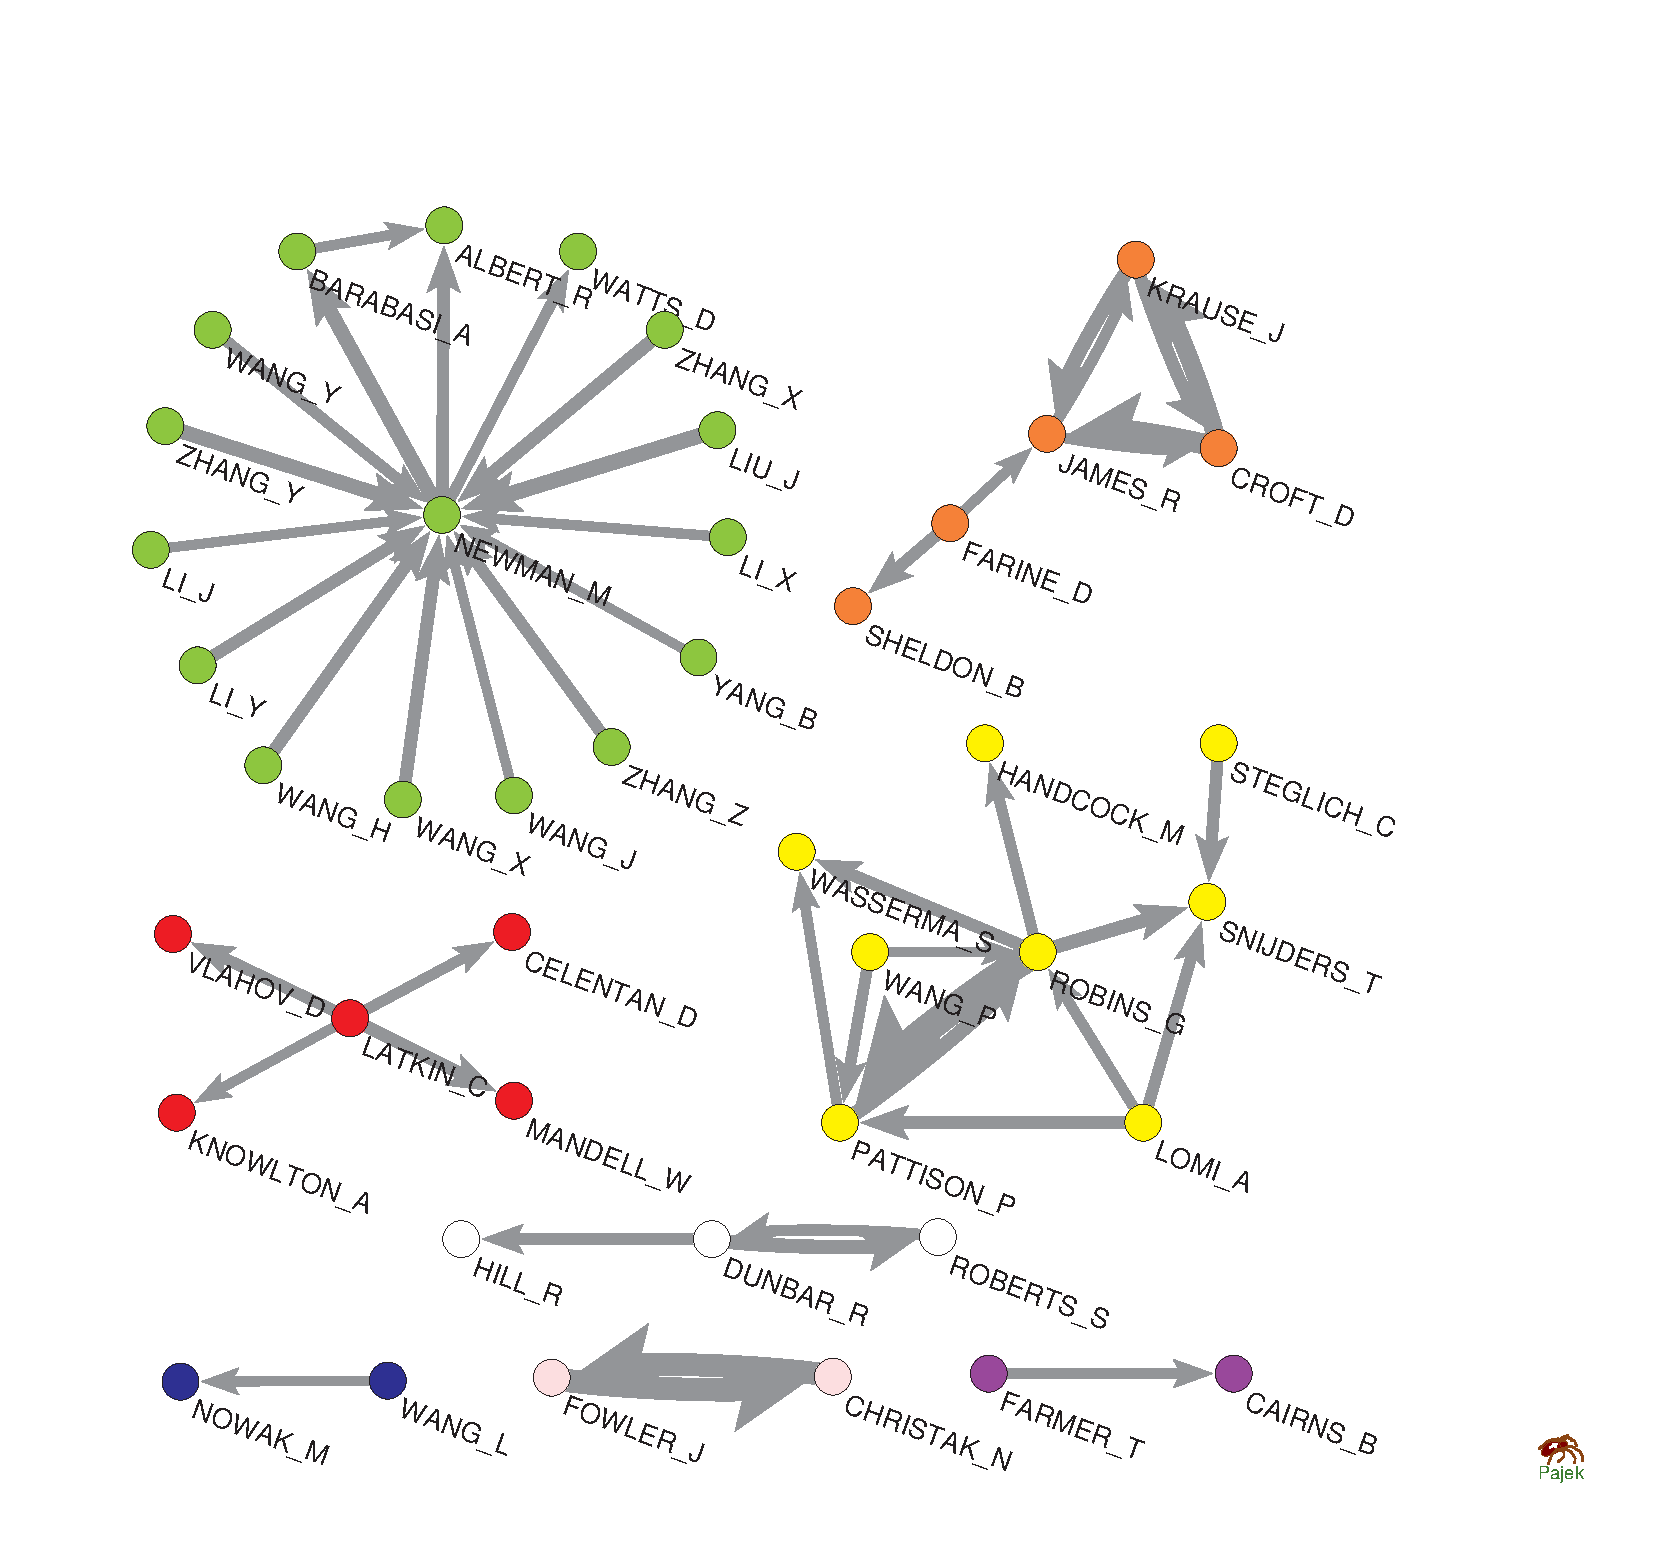
\includegraphics[width=\textwidth]{CiteA_43.pdf}
\end{center}
\caption{CiteA network: Largest line weights} \label{citealw}
\end{figure}

To overcome the overrepresentation of the authors with many works, we used fractional approach. Looking at the \textbf{loops} of the network \textbf{CiteAn}, we can see the highest \textbf{fractional values} of self citations (Table~\ref{authcite}, column ``Value'', again, authors with Chinese and Korean names were excluded).  We also counted \textbf{the proportion} of authors` \textit{self-citations to themselves} and their \textit{external citations to others} by dividing the vector of loops to the vector of outdegree in the CiteAn network (Table~\ref{authcite}, column ``\%''). The proportion of self-citation according to the number of all other citations varies for different authors, however, it is larger for Burt (24\%), Killworth (19\%), Dunbar (18\%), Wellman (17\%), Leydesdorf (17\%), and Atzori (17\%). \medskip  

\begin{table}
\caption{Authors with the highest self-citation} \label{authcite}\medskip
\renewcommand{\arraystretch}{0.99}
\small
\begin{center}
\begin{tabular}{c|l|l|l|l|c|l|l|l|l|} 
\# &	Author & loops &	outdegree & \% &  \# &	Author&  loops &	outdegree & \% \\ \hline 
1	&DUNBAR\_R	&49.34	&274.31	&\textbf{0.18}	      & 21	&FARMER\_T	&11.88	&96.06	&0.12		   \\
2	&LATKIN\_C	&43.23	&508.88	&0.08	      & 22	&CROFT\_D		&11.82	&151.10	&0.08	   \\
3	&JUNG\_J		&29.26	&210.06	&0.14	      & 23	&KILLWORT\_P	&11.00	&59.19	&\textbf{0.19}		   \\
4	&BURT\_R		&25.52	&104.54	&\textbf{0.24}	      & 24	&BERNARD\_H	&10.97	&68.68	&0.16		   \\
5	&CHRISTAK\_N	&24.45	&180.29	&0.14	      & 25	&JAMES\_R		&10.50	&109.82	&0.10	   \\
6	&VALENTE\_T	&24.27	&248.25	&0.10	      & 26	&FRIEDMAN\_S	&10.35	&211.26	&0.05		   \\
7	&BARABASI\_A	&21.48	&143.84	&0.15	      & 27	&ATZORI\_L	&10.15	&59.75	&\textbf{0.17}		   \\
8	&NEWMAN\_M	&20.23	&173.70	&0.12	      & 28	&FARINE\_D	&9.78	&115.99	&0.08		   \\
9	&WELLMAN\_B	&17.08	&99.91	&\textbf{0.17}	      & 29	&EVERETT\_M	&9.34	&69.52	&0.13		   \\
10	&DOREIAN\_P	&16.48	&121.24	&0.14	      & 30	&KRAUSE\_J	&9.03	&99.98	&0.09		   \\
11	&FOWLER\_J	&15.99	&156.65	&0.10	      & 31	&BERKMAN\_L	&8.95	&88.85	&0.10		   \\
12	&SNIJDERS\_T	&13.88	&140.77	&0.10	      & 32	&POTTERAT\_J	&8.90	&88.58	&0.10		   \\
13	&LEYDESDO\_L	&13.80	&78.93	&\textbf{0.17}	      & 33	&MORRIS\_M	&8.86	&110.99	&0.08		   \\
14	&ROTHENBE\_R	&13.46	&145.26	&0.09	      & 34	&KAZIENKO\_P	&8.80	&151.34	&0.06		   \\
15	&RICE\_E		&12.77	&163.03	&0.08	      & 35	&TUCKER\_J	&8.50	&210.81	&0.04		   \\
16	&CARLEY\_K	&12.59	&152.26	&0.08	      & 36	&SKVORETZ\_J	&8.48	&79.38	&0.11		   \\
17	&PATTISON\_P	&12.57	&138.92	&0.09	      & 37	&BATAGELJ\_V	&8.42	&62.48	&0.13		   \\
18	&KELLY\_J		&12.19	&162.15	&0.08	      & 38	&MUTH\_S		&8.38	&125.57	&0.07	   \\
19	&BORGATTI\_S	&11.98	&125.75	&0.10	      & 39	&MARTINEZ\_M	&8.31	&103.10	&0.08		   \\
20	&ROBINS\_G	&11.96	&162.65	&0.07	      & 40	&LITWIN\_H	&8.30	&97.33	&0.09		   \\ \hline 
\end{tabular} 
\end{center}
\end{table}  

We used Islands approach (general) to get islands of the size [5, 200] from the normalized network \textbf{CiteAn} and got 414 islands of size between 5 and 200 (3,418 nodes, or 3.7\% of all the nodes in network). Almost half of these islands (48\%) are of sizes 5 (18\%), 6 (16\%), and 7 (14\%). The largest island Main island of \textbf{CiteAn} network consits of 200 nodes (6\%). We tried to move the upper border of the treshold up to 500 nodes, and it resulted with the Main island of 500 nodes, which means that there is large nested group of nodes. Main island of 200 nodes is presented on the Figure~\ref{CiteAmisl}. In the center there is a group of physicists, surrounded by tje cloud of citations from the `Chinese group'. Most of these authors are again representatived of already mentioned `multiple authors' -- \cite{harzing2015} found them to be highly presented in the field Physics. For the purposes of better visualization, the authors cited Newman, Barabasi separately and both of them together are put to the same place (which produce 3 black lines in the picture). This group also inclues Strogatz, Leskovec, Girvan, Evans.  Left upper part of the graph is consisted of the authors from the Social sciences, traditional representatives of Social network analysis. Among them, the authors with the strongest ties are Borgatti and Everett; the authors having the largest numbders of incoming ties are Freeman (7) is Burt (4); Batagelj also has 2 connections from Ferligoj and Doreian. There is also a trird component of authors positioned around Wasserman, who is being cited by the authors also connected to each other -- Robins and Pattison, Snijders, Holland. Another author citing Wasserman (and Faust) largerly is Kazienko, also having incoming citations (they were also seen in the structures before). Another local star having a lot of incoming ties is Dunbar, having reciprocal connections with Roberts and Pearce. \medskip 

Second and third largest islands are composed of 66 and 41 nodes, respectively. Other islands have  26 and less nodes. Some selected large islands are presented on the Figure~\ref{CiteAislands}. First and second islands (if we count from left to right by three lines) represented by Migliano and Marasco, and Kaskutas, respectively, contain researchers from the fields of medicine, health, desease and addiction. The island of Latkin, Friedman, Potterat, and others was already mentioned above -- this is a group in the field of psychology and health. The group of Chrstakis and Moreno (different ones) represents the researchers working in the field of adolescents, teens in social media, internet addiction, and health. Island formed with Farmer contains researchers working with behavioral and emotional disorders, psychology and youth. Next group represented by Atzori is the one working in the field of internet of things, the one of Folke -- ecology. There is a group of scientists around French sociologist Bourdieu. The group of animal social network analysts Croft, Krause, Farine, and others is quite well-connected. We do not have space and time to drill into all the exported islands, but we can see that there is a large number of groups with different topic specialization. \medskip 

\begin{figure}
\begin{center}
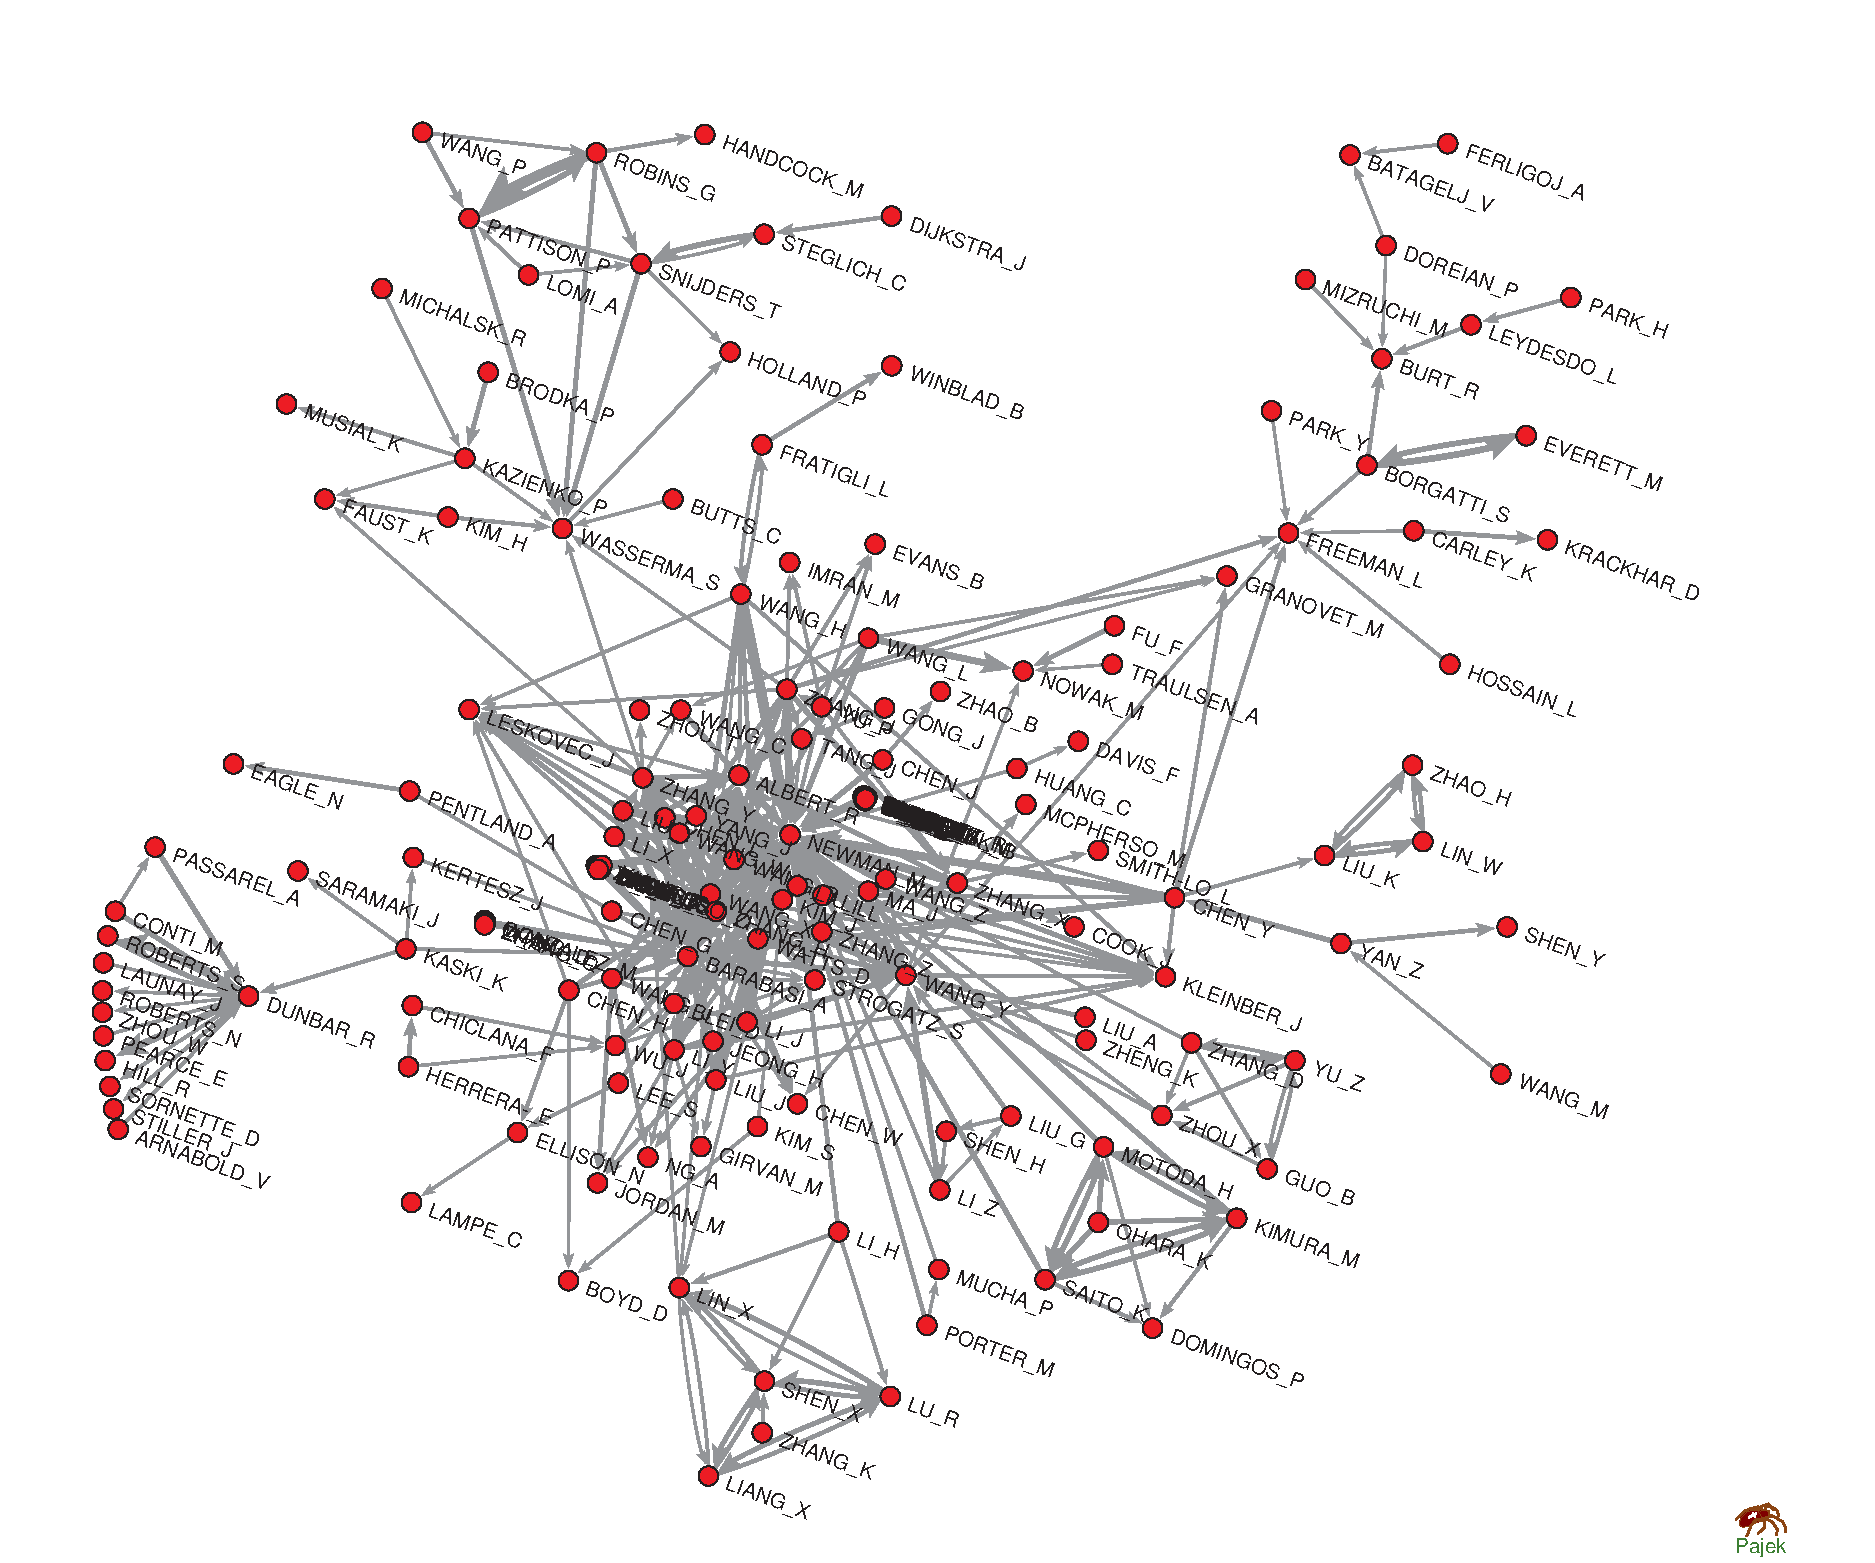
\includegraphics[width=0.7\textwidth]{CiteAmIsl.pdf}
\end{center}
\caption{CiteA:Main island} \label{CiteAmisl}
\end{figure}

\begin{figure}
\begin{center}
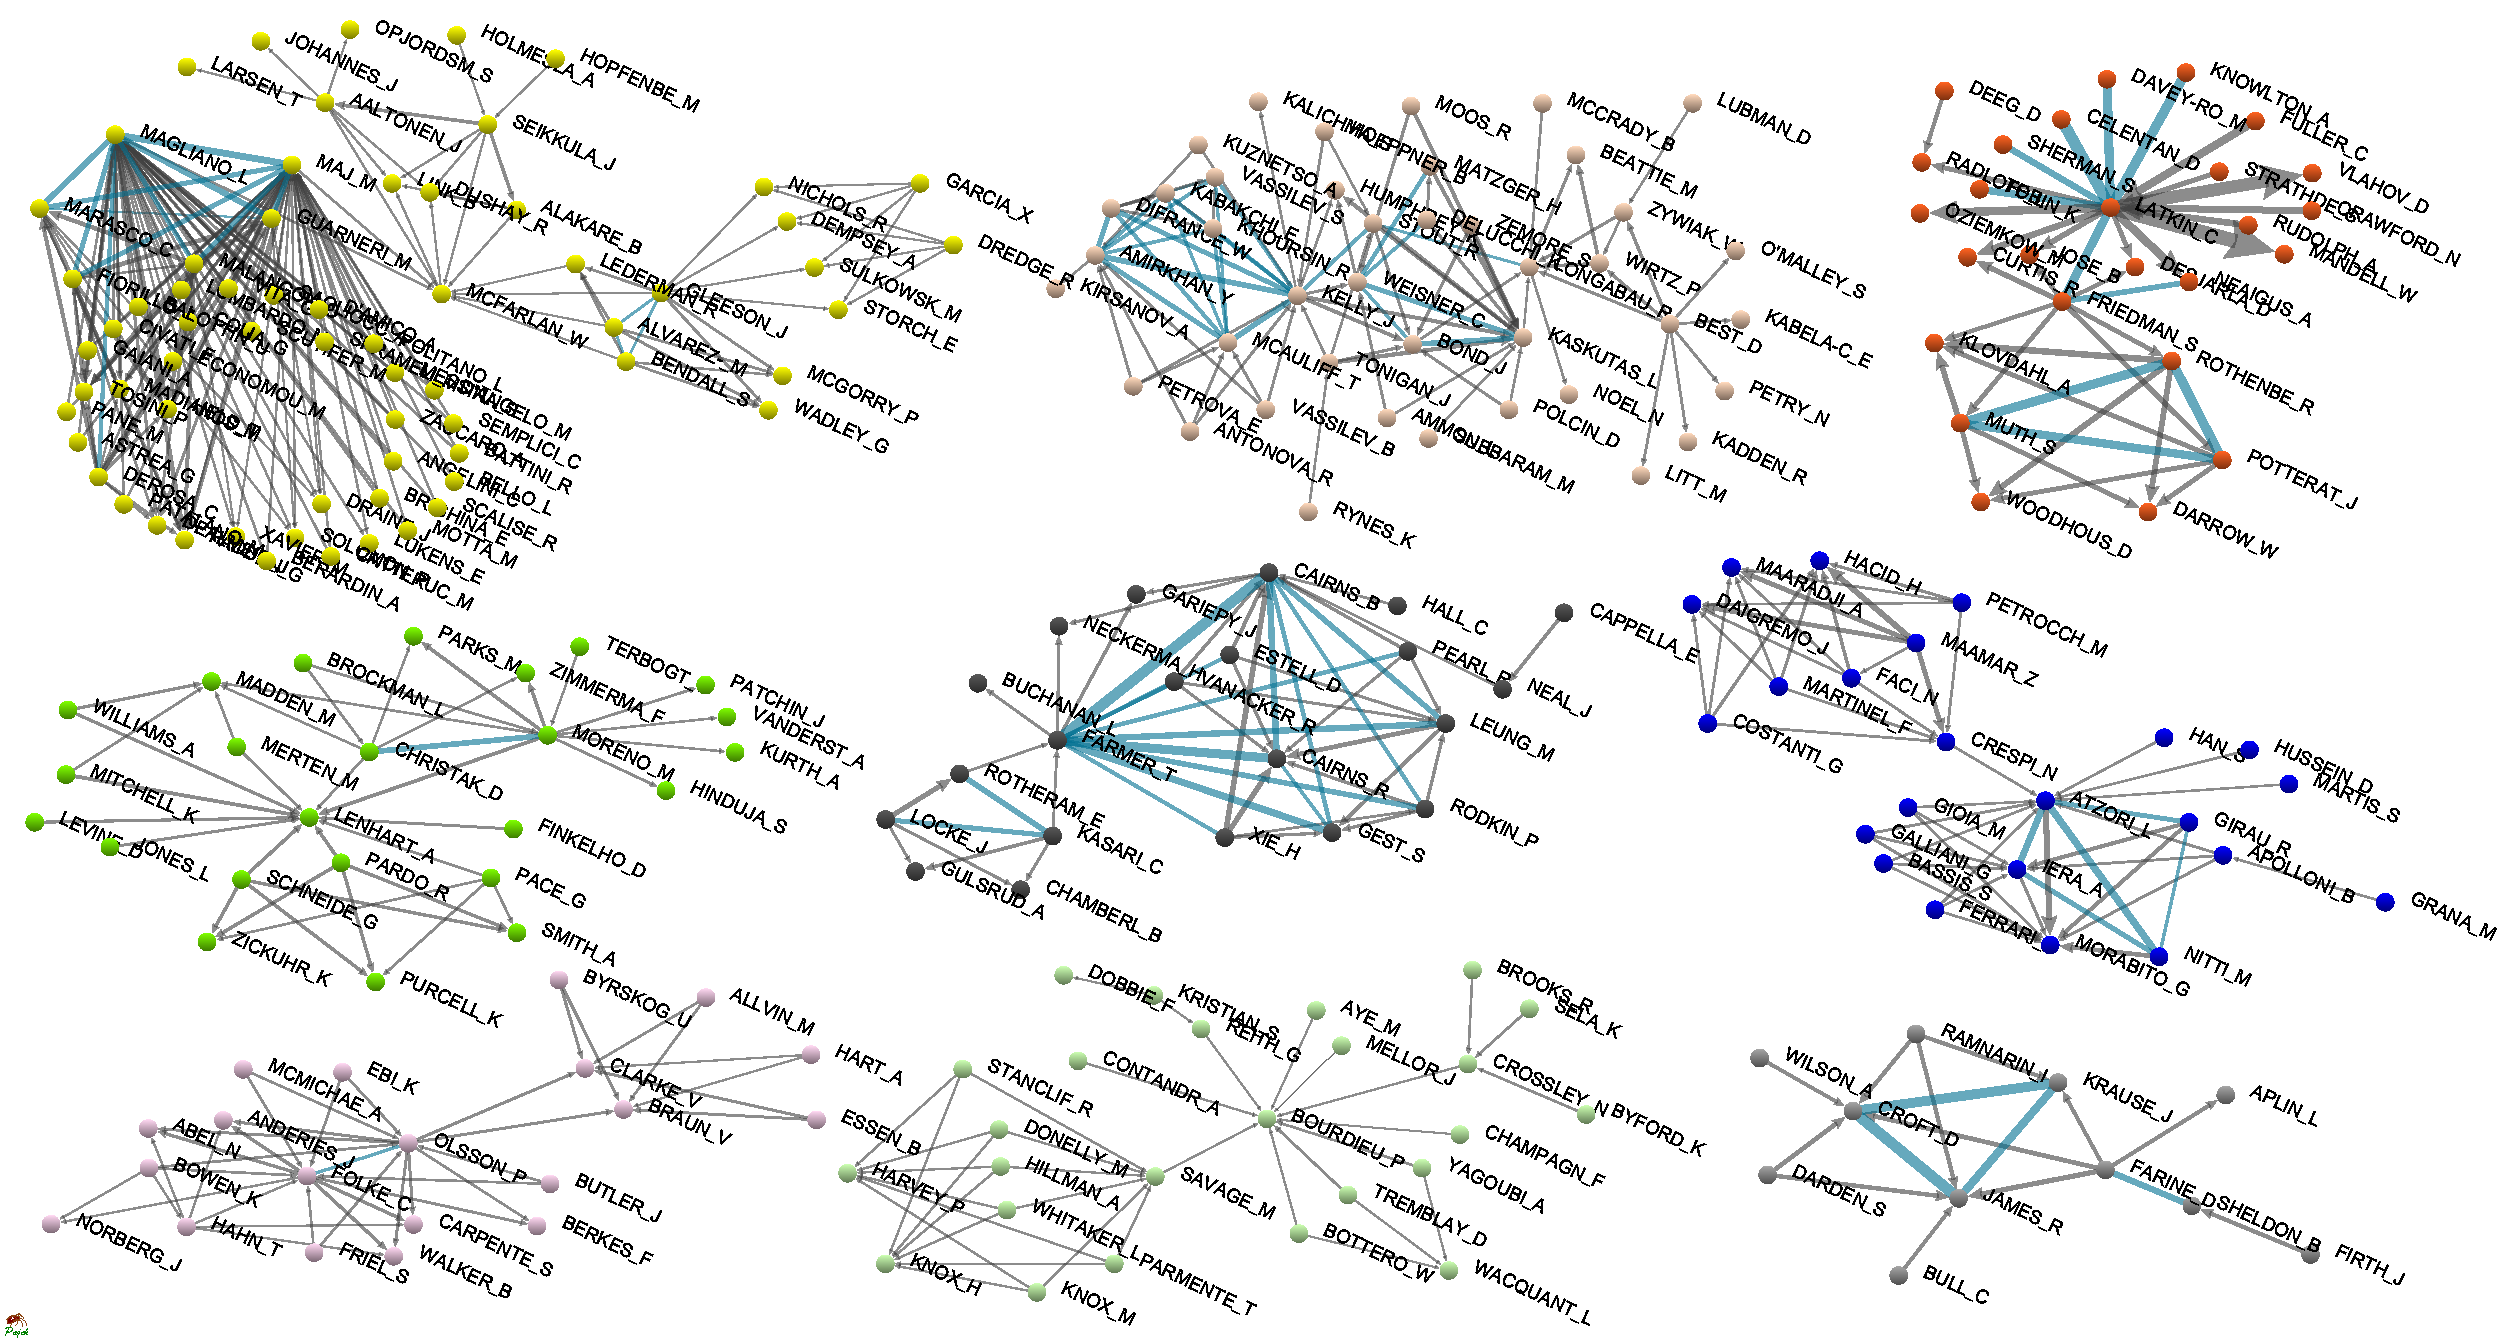
\includegraphics[width=\textwidth]{CiteA_islands.pdf}
\end{center}
\caption{CiteA network: Largest line weights} \label{CiteAislands}
\end{figure}

\section{Citation among journals}

\subsection{Networks creation}

To get information about citations among journals, we computed the \textbf{CiteJ} network, which takes into account citations from papers published in journal \textit{i} to papers published in journal \textit{j}, which appeared in the works included into the \textbf{WJr} network (the analysis was limited to networks with complete descriptions of works). We used a \textbf{CiteR} network to get information on citations between works. In the obtained network, the value of the element $CiteJ[u,v]$ is equal to the \textbf{number of citations} from journal $i$ to journal $j$. \smallskip

\[ \mathbf{CiteJ} = (\mathbf{WJ}) ^ T * \mathbf{Cite} * \mathbf{WJ} \] 

As journals of different sizes were included into the data set, using the \textit{fractional approach} the normalized  $n(CiteR)$ network was also used to produce a \textbf{CiteJn}. The value of the element $CiteJn[u,v]$ is equal to the \textbf{fractional contribution} of citations from papers published in journal $i$ to papers published in journal $j$. \medskip 

\[ \mathbf{CiteJn} = (\mathbf{WJ}) ^ T * n(\mathbf{Cite}) * \mathbf{WJ} \]  
 

\subsection{Citations}

The loops of the \textbf{JJs} network show the journals with the highest \textbf{absolute values} of self citations (Table~\ref{jjloops}). They are \textit{Social Networks} with more then 4,000 citations, and \textit{Computers in Human Behavior} -- with twice less. \textit{Physica A -- Statistical Mechanics and its Applications}, \textit{Physical Review E}, \textit{Lecture notes in Computer Science}, \textit{Cyberpsychology, Behavior, and Social Networking}, and more social sciences oriented \textit{Social Science \& Medicine} and \textit{American Journal of Sociology'} have also relatively high absolute values of citations. \medskip 

After removing loops from the same network, we used a line cut (with a treshold of 205) and extracted the subnetwork of 27 journals with the largest amounts of absolute values of citations given to each other (Figure~\ref{jcij}). The largest component of this network consists of two parts, with \textit{Social Networks} in the center, being largerly cited by the journals from Social sciences, and also citing back the \textit{American Journal of Sociology} and \textit{Journal of Mathematical Sociology}. However, it is also cited a lot from the journals of the second part of the component, belonging to the fields of Natural sciences and general scientific journals -- \textit{Plos One, Lecture Notes in Computer Science, Physica A}. The journals in this part are quite connected with each other. The journal \textit{Computers in Human Behavior} form a separate group, connected to \textit{Cyberpsychology, Behavior, and Social Networking} (reciprocally), as well as to \textit{Journal of Computer-Mediated Communications} and \textit{Personality and Individual Differences}. Another pair of journals are the \textit{Animal Behaviour} citing \textit{Behavioral Ecology and Sociobiology}. 

\begin{table}
\caption{Journals with the highest self-citation: absolute values} \label{jjloops}\medskip
\renewcommand{\arraystretch}{0.95}
\small
\begin{center}
\begin{tabular}{c|l|l} 
 Rank       &        Value   & Id		    \\ \hline 
         1  &    4443   & SOC NETWORKS		    \\
         2  &    2058   & COMPUT HUM BEHAV	    \\
         3  &     569   & PHYSICA A		    \\
         4  &     429   & PHYS REV E		    \\
         5  &     382   & LECT NOTES COMPUT SC	    \\
         6  &     339   & CYBERPSYCHOL BEHAV	    \\
         7  &     328   & SOC SCI MED		    \\
         8  &     315   & AM J SOCIOL		    \\
         9  &     303   & PLOS ONE		    \\
        10  &     258   & ANIM BEHAV		    \\
        11  &     246   & SCIENTOMETRICS	    \\
        12  &     232   & J MED INTERNET RES	    \\
        13  &     226   & P NATL ACAD SCI USA	    \\
        14  &     209   & ORGAN SCI		    \\
        15  &     194    & BEHAV ECOL SOCIOBIOL	     \\ \hline 
\end{tabular} 
\end{center}
\end{table}  

\begin{figure}
\begin{center}
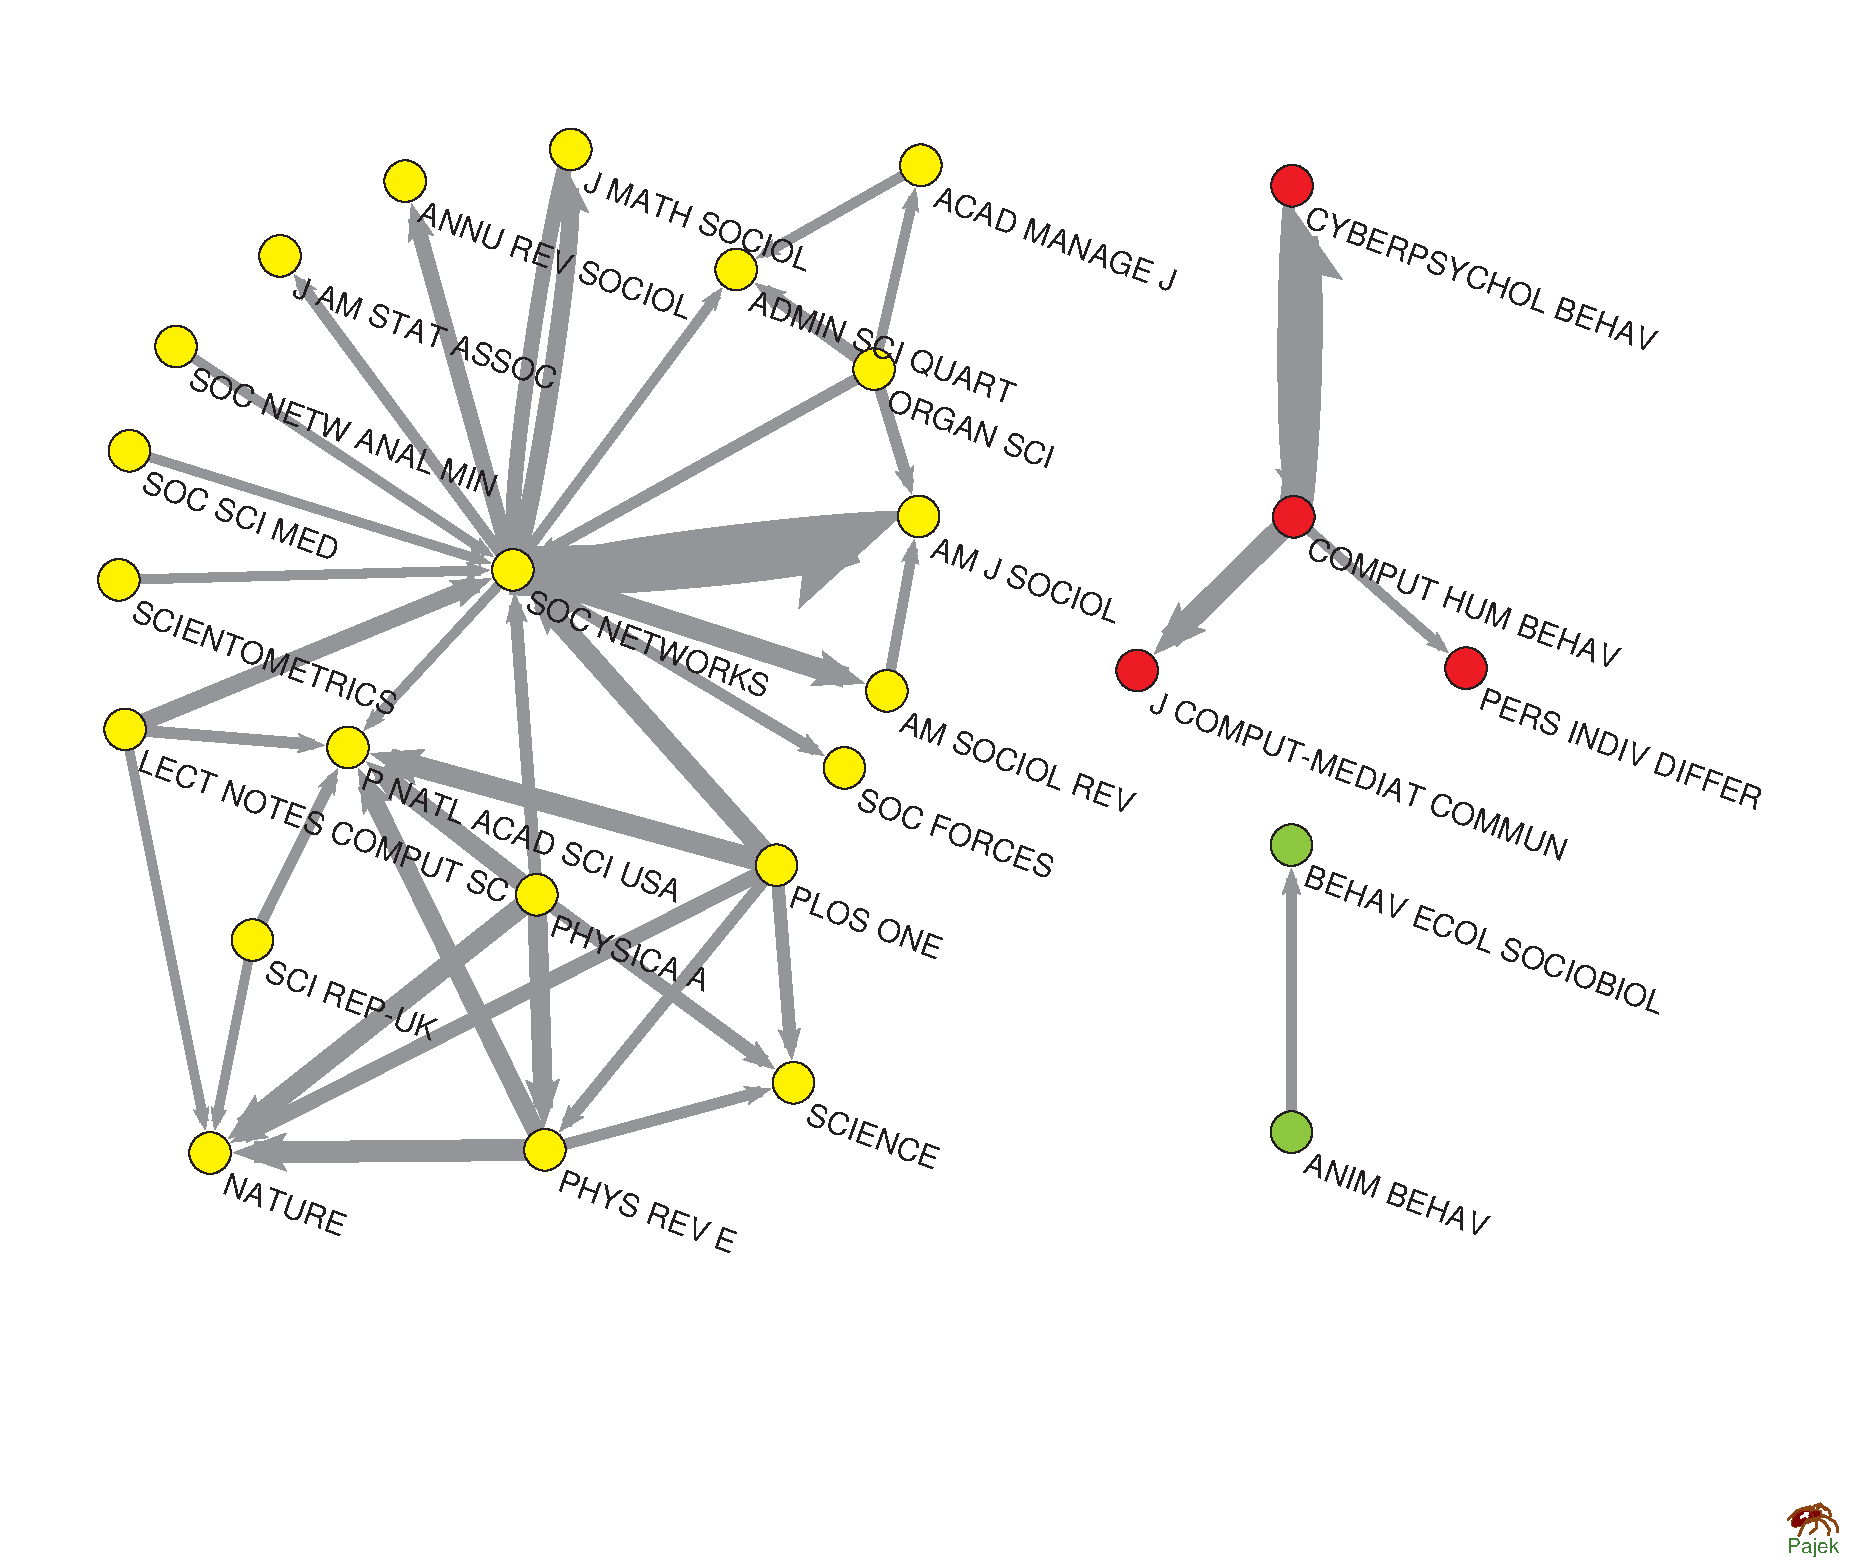
\includegraphics[width=150mm]{JCiJ_27.pdf}
\end{center}
\caption{JCiJ network: Largest line weights} \label{jcij}
\end{figure}
\medskip

The loops of the \textbf{JJsfn} network show the journals with the highest \textbf{fractional values} of self-citations (Table~\ref{jselfcite}, column ``Value''). Even though some level of self-citation is is typical for all journals, there are some journals that have larger levels. Again, the highest value belongs to the \textit{Social Networks} journal. Other highly ranked journals are from the fields of Computer science and Cyberpsychology -- the journals \textit{Computers in Human Behavior} and \textit{Lecture Notes in Computer Science} (the previous order is a bit changed). Other journals with relatively high number of internal citations are already mentioned before \textit{Physica A, Social Science \& Medicine}, \textit{Cyberpsychology, Behavior, and Social Networking}, as well as {Journal of Medical Internet Research}, which appears in the table above on a lower place. The differences between values for the first three listed journals and others are quite significant. \medskip 

However, as different journals have different number of works, we also counted \textbf{the proportion} of journals` \textit{internal citations to themselves} and their \textit{external citations to other journals} by dividing the vector of loops to the vector of outdegree in the JJsfn network (Table~\ref{jselfcite}, column ``\%''). Several journals with the highest values -- \textit{Nature, American Journal of Sociology, American Journal of Epidemiology, Journal of Medical Internet Research, Comunicar Journal} -- have quite high level of internal citation -- around the quarter. \textit{Social Networks} journal has even more -- 34\% of internal citations.  Large level of citation within a journal to the same journal may mean that it is seen as an important source of information for the scientists involved into the particular field.\medskip 

\begin{table}
\caption{Journals with the highest self-citation} \label{jselfcite}\medskip
\renewcommand{\arraystretch}{0.95}
\small
\begin{center}
\begin{tabular}{c|l|l|l|c|l|l|l|} 
\# &	Value& \% &	Journal &  \# &	Value& \% & Journal \\ \hline 
1 &	\textbf{355.65}&	\textbf{0.34}&	SOC NETWORKS&	16&	       18.35 &    0.17	  &     ANIM BEHAV\\
2 &	\textbf{168.39}&	0.22&	COMPUT HUM BEHAV&	17&    17.03 & 	  0.12	  &     AIDS BEHAV\\
3 &	\textbf{122.57}&	0.09&	LECT NOTES COMPUT SC&	18&    16.03 & 	  0.19	  &     AM J COMMUN PSYCHO \\
4 &	57.75&	0.13&	PHYSICA A&	19&	       14.87 &	  0.10	  &     INFORM SCI\\
5 &	43.00&	0.14&	SOC SCI MED&	20&	       14.14 &	  0.14	  &     KNOWL-BASED SYST\\
6 &	42.18&	\textbf{0.24}&	J MED INTERNET RES&	21&    12.64 &	  0.19	  &     PROF INFORM\\
7 &	41.49&	0.21&	CYBERPSYCHOL BEHAV&	22&    12.35 & 	 \textbf{0.23}	  &     COMUNICAR\\
8 &	33.16&	0.05&	PLOS ONE&	23&	       12.00 & 	  0.18	  &     BEHAV ECOL SOCIOBI \\
9 &	32.93&	0.11&	PHYS REV E&	24&	       11.87 & 	  \textbf{0.25}	  &     AM J EPIDEMIOL\\
10 &	30.22&	0.13&	SCIENTOMETRICS&	25&	       11.01 & 	  0.11	  &     DECIS SUPPORT SYST \\
11 &	24.16&	0.14&	P NATL ACAD SCI USA&	26&    10.58 & 	  0.14	  &     J ETHN MIGR STUD\\
12 &	23.15&	\textbf{0.26}&	AM J SOCIOL&	27&	       10.43 & 	  0.13	  &     COMPUT EDUC\\
13 &	20.04&	0.05&	LECT NOTES ARTIF INT&	28&    10.31 & 	  0.18	  &     SEX TRANSM DIS\\
14 &	19.31&	0.12&	EXPERT SYST APPL&	29&    10.19 & 	 \textbf{0.28}	  &     NATURE\\
15 &	18.77&	0.14&	NEW MEDIA SOC&	30&	       9.85 & 	  0.09	  &     ORGAN SCI\\ \hline 
\end{tabular} 
\end{center}
\end{table}  

We generated Islands of size between 2 and 5, and got 193 islands, with the largest island containing 50 nodes. The Main islands is presented on the Figure~\ref{jjFmain1}.Citations among journals have clear acyclic (hierarchical) organization. There can be sevral main groups of journals detected: journals in Social Sciences (on the right), Computer Science (on the left), Physics (in the middle) and General scientific journals (in the bottom).  \medskip 

In the \textbf{Computer Science group} of journals, the most citing position is taken by \textit{Lecture Notes in Computer Science}, which largerly cite the journals from all the groups: Computer Science (\textit{Computer Networks, Communications of the ACM, Computers in Human Behavior}, and others), Social sciences (\textit{Social Networks, Social Network Analysis and Mining, Structural Analysis in the Social Sciences, Annual Review of Sociology}), Physics (\textit{Physical Review}, and General scientific journals (\textit{Nature, Journal of Interdisciplinary Sciences, Proceedings of the National Academy of Sciences USA}. It also have equal number of outgoing and incoming citations with the journal \textit{Lecture Notes in Artficial Intelligence}, which also cites a lot of journals from different fields. Another journal from this group -- \textit{Computers in Human Behavior} -- is largerly citing the journal \textit{Cyberpsychology, Behavior, and Social Networking}, which also cites it back, \textit{Journal of Computer-Mediated Communication}, and other journals related to Behavioral studies and Information Systems, as well as Media. \medskip 

The group of journals from the \textbf{Physics} is presented by only three journals -- \textit{Physica A -- Statistical Mechanics and Its Applications, Physical Review E, Physical Review Letter}, with the first one citing others. The \textit{Physica A, Physical Review E} are also the journals that cite largerly general scientific journals \textit{Nature} and \textit{Science}. It is also seen that the traditional, older \textbf{general scientific journals} -- \textit{Nature, Science, Journal of Interdisciplinary Sciences, Proceedings of the National Academy of Sciences USA} are cited by the newly emerged one -- \textit{Plos One}. \medskip  

In the \textbf{Social Sciences group}, the most citing journal is \textit{Social Networks}, which is strongly connected to the \textit{Amercian Journal of Sociology}, as well as have outgoing connections to many other sociological journals (\textit{Journal of Mathematical Sociology, Social Forces, American Sociological Review, Social Network Analysis and Mining}, which also cite it back (however, in a less degree), and \textit{Annual Review of Sociology, Sociological Methodology}. This \textit{Social Networks} journal is also cited by other journals from differnt fields of Social sciences (Sociology, Organizational science, Information science, Methodology), as well as from the journals of the two mentioned above groups. For this journal, the largest incoming citatons go from \textit{Lecture Nodes of Computer Science,  Lecture Notes in Artficial Intelligence, Plos One, Physica A}. Thus, the journal itself cites mostly journals from the field of Social sciences, but it is being cited by the journals from other disciplines -- Computer, Physics, and General scientific fields. There are also links from \textit{Lecture Notes in Computer Science} and \textit{Plos One} to  the \textit{American Journal of Sociology}. \medskip  \medskip 

Other 29 obtained islands of journals citing each other sized from 3 to 6 (107 nodes) are the ones on the topics of: psychology and deviation;  psychiatry; medicine; surgery; health disabilities; substance abuse and addiction; nursering; social work; archeology and anthropology; language and sociolinguistics; economics and economic behavior; education; conflicts and peacekeeping; library science; ergonomics; transportation. There are also three journals from the field of behavioral ecology and animal behavior: \textit{Behavioral Ecology and Sociobiology} being cited by \textit{Animal Behaviour} and \textit{Behavioral Ecology}. \medskip 
 
%\begin{figure}
%\begin{center}
%\includegraphics[width=0.9\textwidth,viewport=35 0 965 
%740,clip=]{JJfMain.pdf}
%\end{center}
%\caption{Citations among journals -- main island} \label{jjFmain}
%\end{figure}

\begin{figure}
\begin{center}
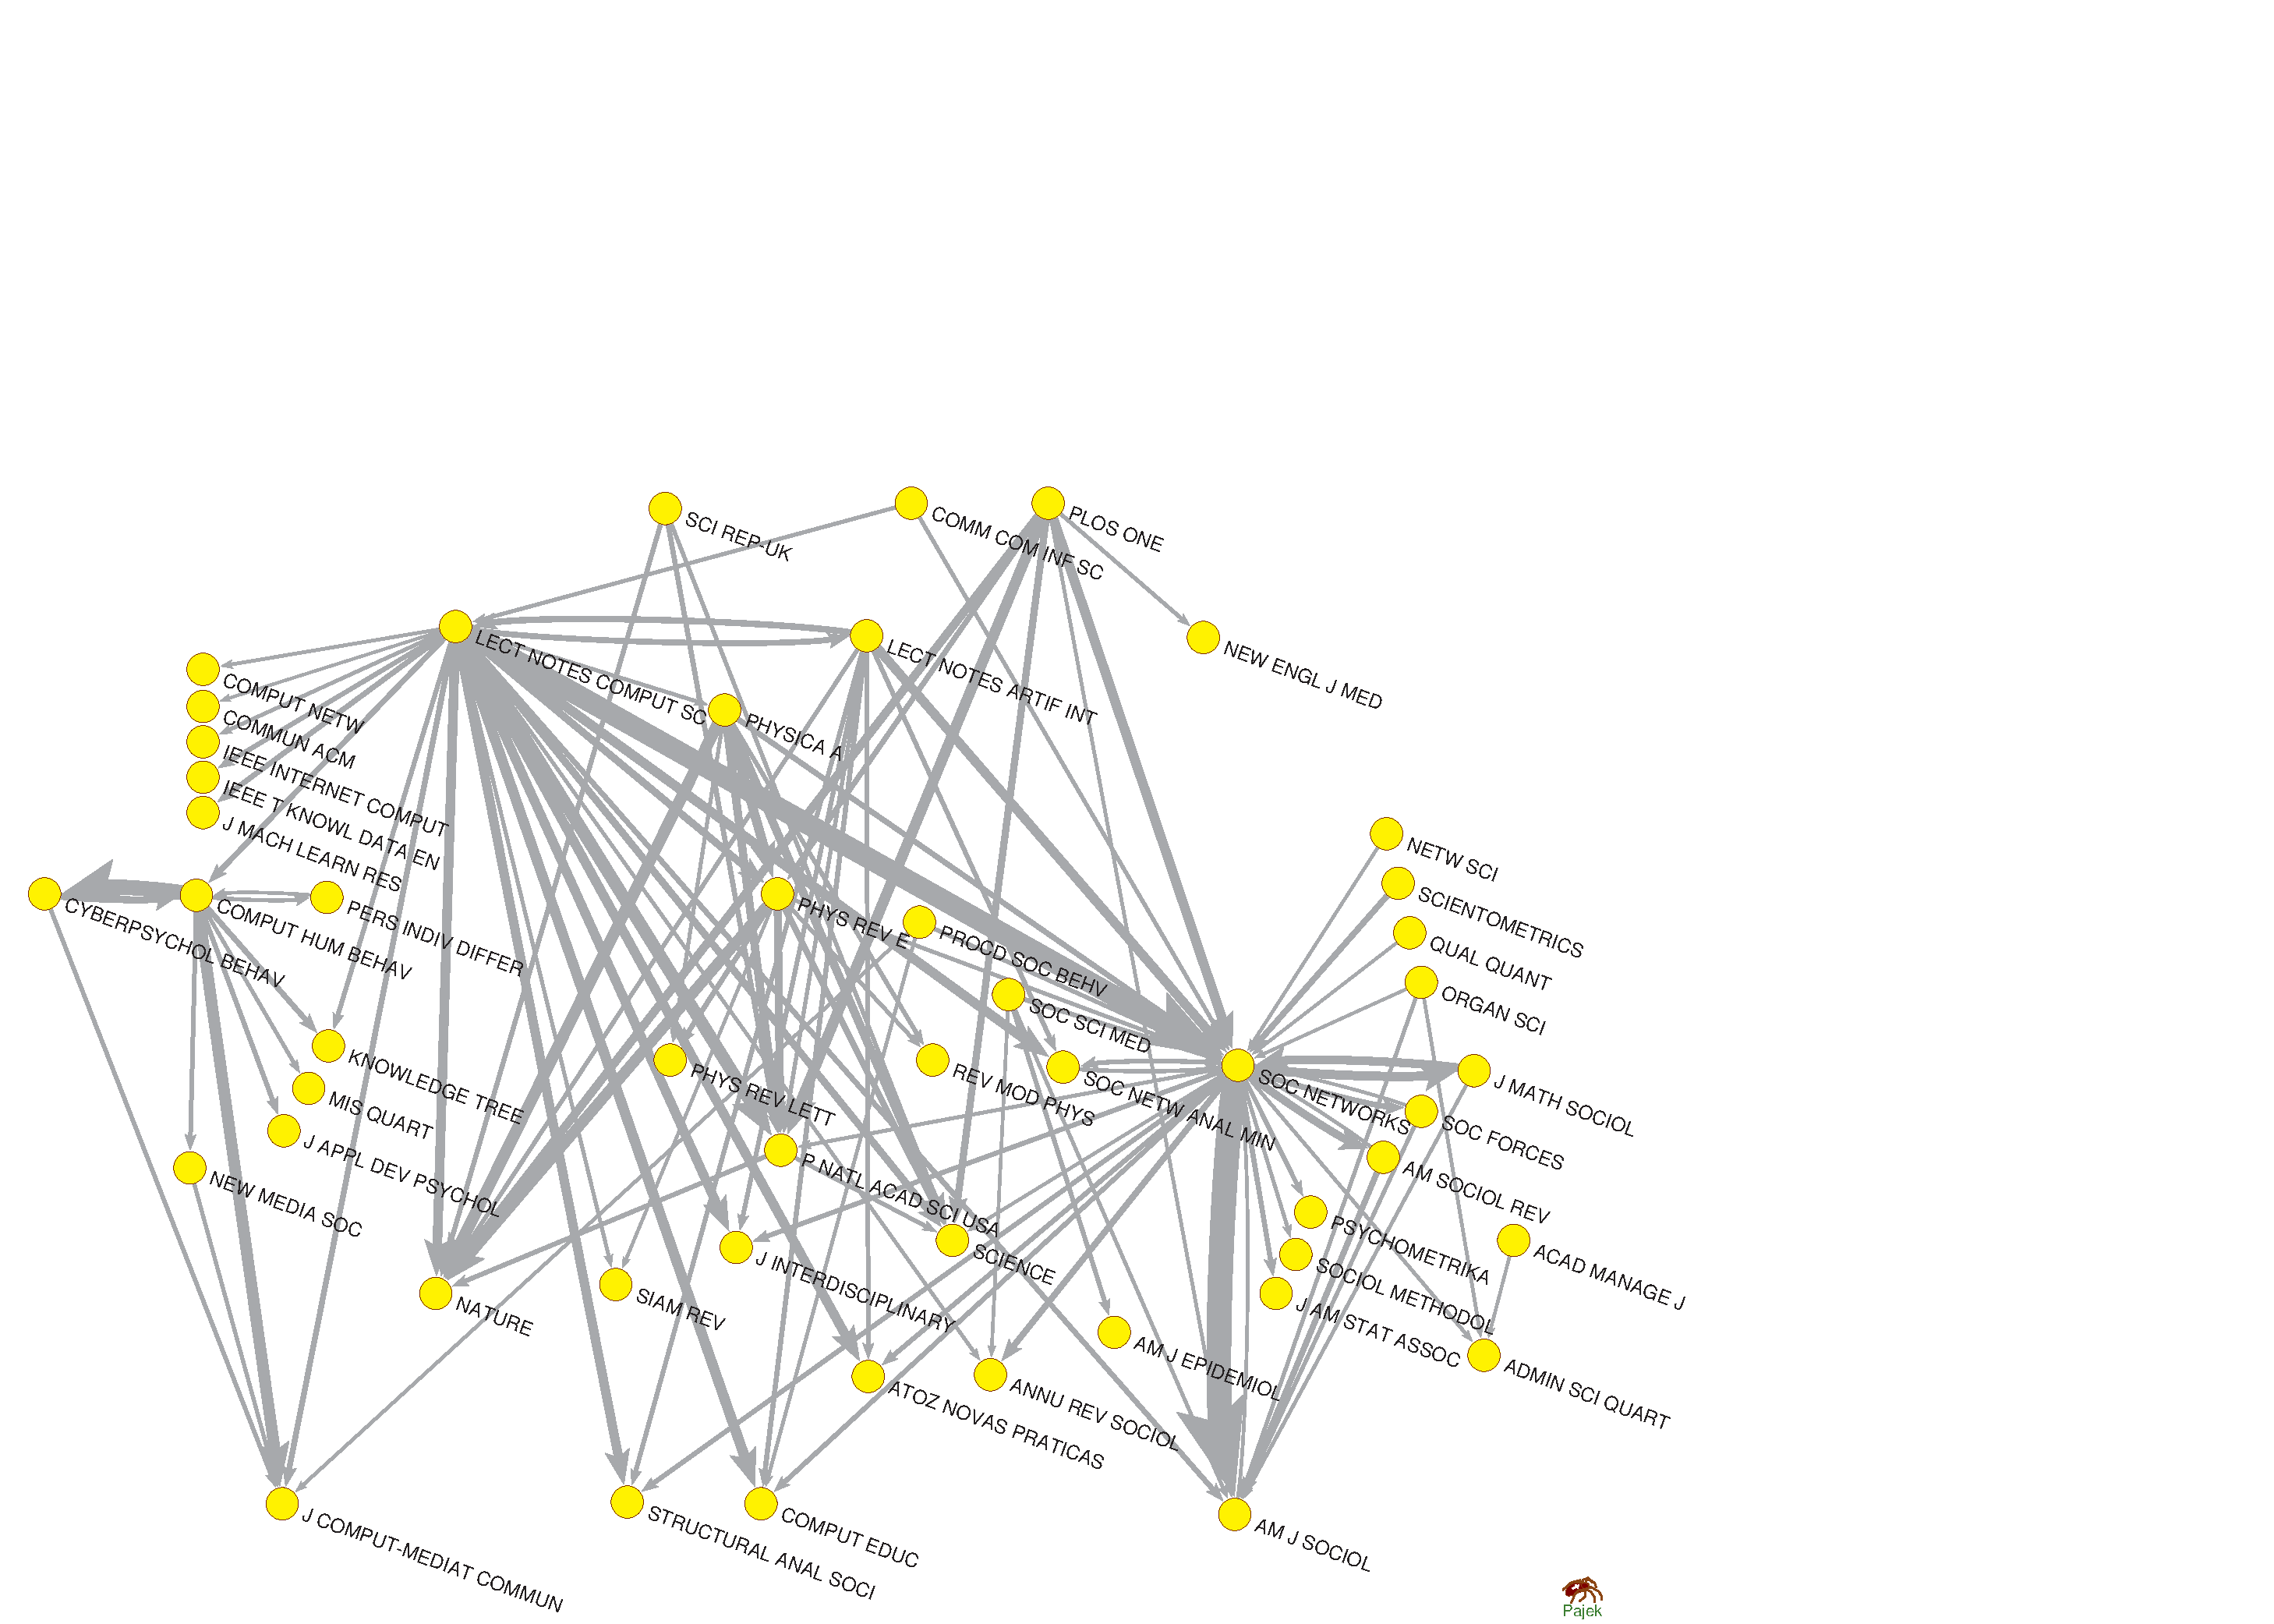
\includegraphics[width=0.9\textwidth,viewport=10 0 1045 705
740,clip=]{JJsfmain2.pdf}
\end{center}
\caption{Citations among journals -- Main island} \label{jjFmain1}
\end{figure}

Other islands 31-193 contain (326 nodes) only 2 nodes -- they are pairs of journals. Journals with the largest weights of lines are presented on the Table~\ref{jpairs}. The links are directed: first written journal cites second one. These journals cover the wide range of topics, including \textit{health, health policy, psychology and psychiatry, adolescence, sex, STD and AIDS, migration, communication, demography,  business and management, consuming behavior and marketing, information science, computing, language,  peace and conflicts, engineering}. 

\begin{table}
\caption{Pairs of journals} \label{jpairs}\medskip
\renewcommand{\arraystretch}{0.9}
\small
\begin{center}
\begin{tabular}{c|l|p{5cm}|p{5cm}|}
\# &	value &	from journal  &	to journal \\  \hline 
1&	8,1&	IEEE GLOB COMM CONF&	IEEE INFOCOM SER\\
2&	6,26&	HIST COMUN SOC&	COMUNICAR\\
3&	4,63&	J YOUTH ADOLESCENCE&	J RES ADOLESCENCE\\
4&	4,44&	INT J GERIATR PSYCH&	J PSYCHIAT RES\\
5&	4,38&	INT MIGR&	INT MIGR REV\\
6&	4,31&	J BUS ETHICS&	ACAD MANAGE REV\\
7&	3,99&	DEMOGR RES&	DEMOGRAPHY\\
8&	3&	J INTELL FUZZY SYST&	J APPL MATHE COMPUT\\
9&	3&	J INT DEV&	TROP MED INT HEALTH\\
10&	3&	PERVASIVE MOB COMPUT&	INT CONF PERVAS COMP\\
11&	2,78&	J CONSTR ENG M&	J CONSTR ENG M ASCE\\
12&	2,68&	PHYS EDUC RES CONF&	PHYS REV SPEC TOP-PH\\
13&	2,59&	ENERGY RES SOC SCI&	ENERG POLICY\\
14&	2,5&	INT P ECON DEV RES&	TECHNOVATION\\
15&	2,37&	COMPUT ASSIST LANG L&	LANG LEARN TECHNOL\\
16&	2,33&	INFORM SOC-ESTUD&	PERSPECT CIENC INF\\
17&	2,33&	WORLD DEV&	ECON J\\
18&	2,31&	J PEACE RES&	J CONFLICT RESOLUT\\
19&	2,22&	HEALTH RES POLICY SY&	HEALTH POLICY PLANN\\
20&	2,1&	SEX HEALTH&	INT J STD AIDS\\
21&	2&	REV LAT COMUN SOC&	PALABRA CLAVE\\
22&	2&	J RETAIL CONSUM SERV&	AUSTRALAS MARK J\\
23&	2&	ETHN DIS&	HEART LUNG\\
24&	2&	IEEE INT SYMP INFO&	IEEE T INFORM THEORY\\
25&	2&	REV BRAS ENFERM&	REV LAT-AM ENFERM\\ \hline 
\end{tabular}
\end{center}
\end{table}  


\section{Bibliographic Coupling}

\subsection{Networks creation} 

Bibliographic coupling occurs when two works each cite a third work in their bibliographies -- and this suggests some content communality between these two works. Having more works citing pairs of prior works increases the likelihood of them sharing content [Batagelj, chapter 2]. We used \textbf{CiteR} network to produce a \textbf{Jaccard biCo} network, which can be determined as: 

\[ \mathbf{biCo} = \mathbf{Ci} * (\mathbf{Ci}) ^ T \]  

\[ \mathbf{biCo_{pq}} = \textrm{\# of works cited by both works p and q} = \mid Ci(p) ...  Ci(q) \mid \]  

Bibliographic coupling weights are symmetric: biCopq = biCoqp:

\[ \mathbf{biCo}^T = (\mathbf{Ci} * \mathbf{Ci} ^ T ) ^ T = \mathbf{Ci} * \mathbf{Ci}^T = \mathbf{biCo} \] 

Using obtained network, we constructed two networks -- co-citations between journals \textbf{JCoj} and co-citations between authors \textbf{ACoj} -- by its multiplication with normalized \textbf{WJsr} and \textbf{WAsr} networks (we limited our analysis to networks with complete descriptions of works).  Normalization creates networks $n(WJr)$ and $n(WAr)$ where the weight of each arc is divided by the sum of weights of all arcs having the same initial node (journal or author) as this arc (outdegree of a node). Weights in the obtained networks take into account \textit{fractional} similarity of journals $i$ and $j$, or authors $u$ and $v$.  \medskip

\[ \mathbf{JCoj} = n(\mathbf{WJ}) ^ T * \mathbf{biCoj} * n(\mathbf{WJ}) \]  

\[ \mathbf{ACoj} = n(\mathbf{WA}) ^ T * \mathbf{biCoj} * n(\mathbf{WA}) \]  

The values of links from biCoj are redistributed in JCoj and ACoj. The total sum of link weights is preserved.

	\[ \sum_{e \in E(\mathbf{JCoj})} \mathbf{JCoj}[e] = \sum_{e \in E(\mathbf{biCoj})} \mathbf{biCoj}[e] \] 

We should note that the produced Jaccard network \textbf{biCo} contained a large number of links -- 62.079.457, -- and that`s why the computation of networks \textbf{JCoj} and \textbf{ACoj} would be quite time consuming. That`s why the desision was made to make a link cut in the Jaccard \textbf{biCo} at the level 0.085, and then use the obtained network for the multiplication with \textbf{WJsr} and \textbf{WAsr} networks, respectively. \Remark{change: full Jaccard network size, obtained networks sizes} The obtained \textbf{biCo} network contained 70.792 works and 13.208.451 links (change). After multiplication, we got \textbf{JCoj} network with 8.943 nodes and 4.966.617 arcs (including XXX loops), and \textbf{ACoj} network with 93.011 nodes and 127.220.243 arcs (including 14.131 loops). In both obtained networks, the loops were deleted, the bidirected arcs were converted to edges (with summation of values) before the further analysis.\medskip

\subsection{Co-citation among journals} 

After simplification, \textbf{JCoj} network contained 8,943 nodes and 5,136,616 edges. However, the majority of lines was of a very low value, and after the line cut at the level 1200 (as journals have great weights, a large link-cut was required), we got a network of 41 nodes. \medskip

Most of the journals presented on the Figure~\ref{jacj} are journals from the fields of Physics and Computer science closely connected to each other, which means -- sharing the large amount of literature in their citations. Four such journals are particularly prominent: \textit{Physica A, Physical Review E, Lecture Notes in Computer Science} and \textit{Lecture notes in artificial intelligence}, with \textit{Plos One}, representing general scientific journals. These results are similar to the ones obtained for the analysis of literature on clustering [Batagelj, Chapter 2]. \textit{Social Networks} journal is also presented, having connections (and similar citation patterns) with all journals mentioned above as well as with journals from the group of \textit{Social Sciences} -- \textit{Journal of Mathematical Sociology, Social Forces, American Sociological Review, American journal of Sociology, Social Science \& Medicine} and \textit{Scientometrics}. It does not have conections to \textit{Social Network Analysis and Mining} journal -- despite its name, it is focused more on data mining in large networks and reflects more a computer science orientation.

\begin{figure}
\begin{center}
\includegraphics[width=110mm]{JacJ_43.pdf}
\end{center}
\caption{Cj network: Journals} \label{jacj}
\end{figure}

\subsection{Co-citation among authors} 

To make the obtained \textbf{ACoj} network manageble for the analysis, the line cut at the level 2.5 was done at first, and the network of 1.162 nodes and  9.926 arcs (including 402 loops) was obtained. After simplification, we got the network with same number of nodes and 4.762 of edges. We used Islands approach (regular islands) and extracted 9 islands of sizes from 5 to 40. These islands are presented in the Figure~\ref{jaca}.  \medskip 

The larger island on the left comes from the physics driven literature and is centered on Newman. Most of the authors in this island are again Chinese authors, but it also includes such well-known physicists as \textit{Barabasi, Albert, Watts} and \textit{Strogatz}. The second and third islands contains sets of traditional social network scientists. In the second island, among 17 scientists the largest indegree weights are taken by \textit{Burt, Doreian, Bonachich, Everett, Borgatti}. In the third island, the most central are \textit{Robins, Pattison} and \textit{Snijders}. The last island shows the similarity in citation patterns between authors from the field of animal social network analysis. There are five more islands of star-like structures, with \textit{Berkman, Dunbar, Kaskutas, McClurg, R.White} in the center. 

\begin{figure}
\begin{center}
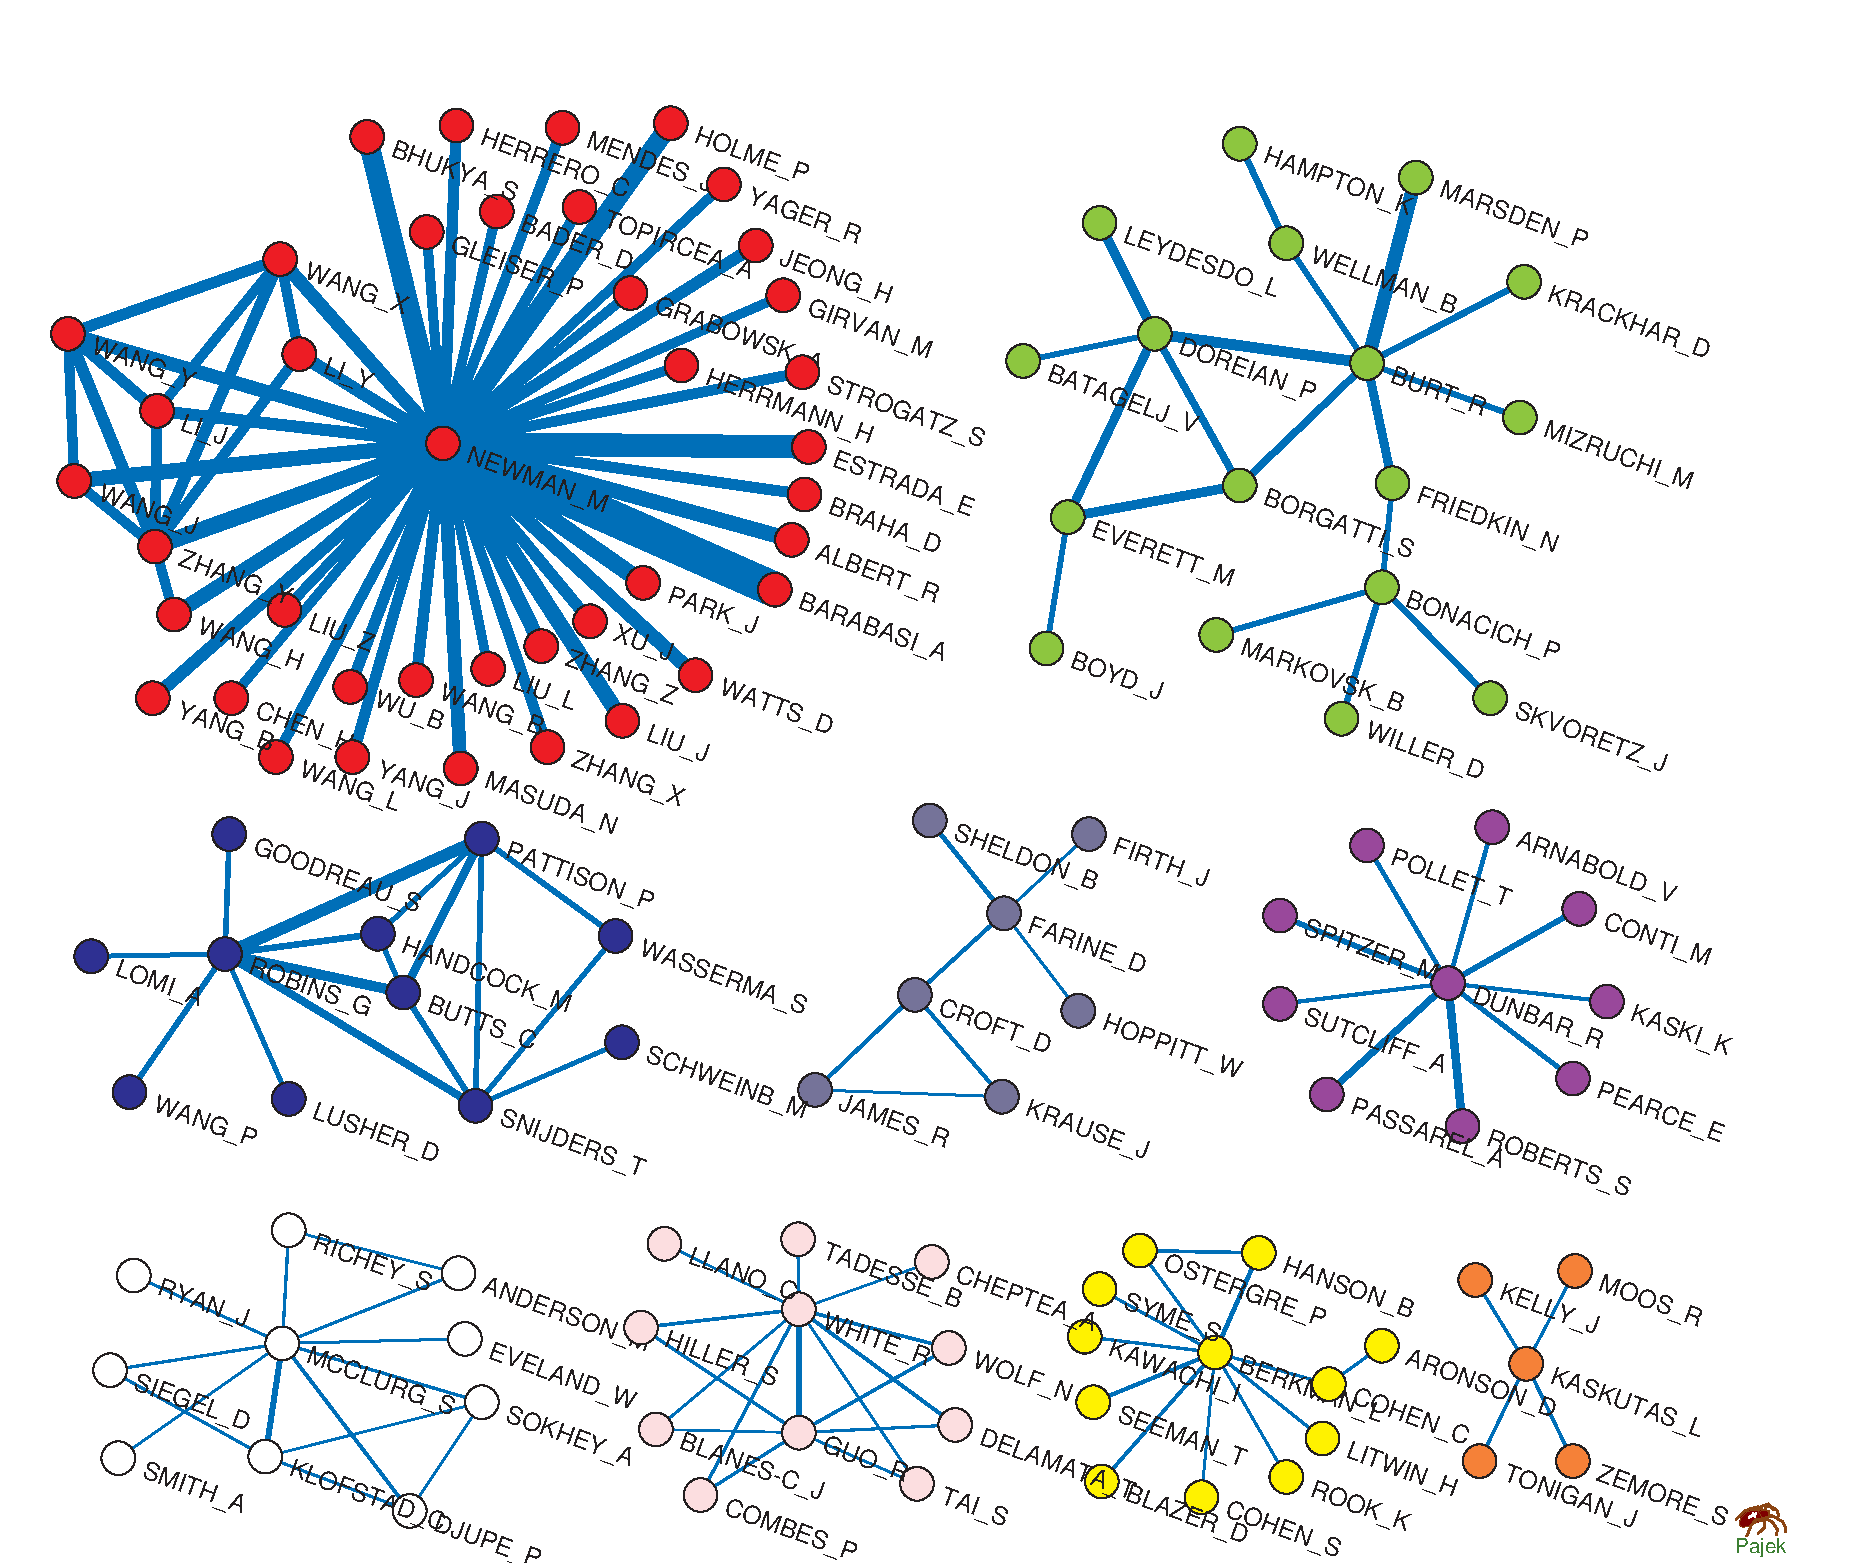
\includegraphics[width=110mm]{JacAu.pdf}
\end{center}
\caption{Jaccard network: Authors} \label{jaca}
\end{figure}

%******************************************************************************



%******************************************************************************
\section{Conclusions}



%******************************************************************************

\begin{thebibliography}{99}
\bibitem[Barabasi et al.(2002)]{Evol}
   Barabâsi, A. L., Jeong, H., Néda, Z., Ravasz, E., Schubert, A., Vicsek, T. (2002). Evolution of the social network of scientific collaborations. Physica A: Statistical mechanics and its applications, 311(3-4), 590-614.
\bibitem[Batagelj(2008)]{sn5}
   Batagelj V. (2005). SN5 -- network data for Viazards session at INSNA Sunbelt 2008. http://vlado.fmf.uni-lj.si/pub/networks/data/WoS/SN5.zip      
\bibitem[Batagelj(2017)]{wos2pajek}
   Batagelj, V. (2017) WoS2Pajek. Networks from Web of Science. Version 1.5 (2017). URL: http://vladowiki.fmf.uni-lj.si/doku.php?id=pajek:wos2pajek 
\bibitem[Batagelj and Cerinšek(2013)]{OnBibl}    
   Batagelj V., Cerinšek M.(2013). On bibliographic networks. Scientometrics. 96 (3), 845-864
\bibitem[Batagelj(2014)]{arxiv}  
   Batagelj, V. (2014) Efficient Algorithms for Citation Network Analysis. arXiv:cs/0309023 
\bibitem[Batagelj et al.(2014)]{Understand}
   Batagelj, V., Doreian P., V., Ferligoj, A., Kejžar N. (2014). Understanding Large Temporal Networks and Spatial Networks: Exploration, Pattern Searching, Visualization and Network Evolution. 
\bibitem[Batagelj et al.(2017)]{PeerRew}    
   Batagelj, V., Ferligoj, A. Squazzoni, F. (2017) The emergence of a field: a network analysis of research on peer review. Scientometrics,  113: 503. https://doi.org/10.1007/s11192-017-2522-8  
\bibitem[Batagelj et al.(2019)]{batagelj2019}
   Batagelj V., Ferligoj A., Doreian P. (2019). Bibliometric analysis of the network clustering literature. In Doreian P., Batagelj V., Ferligoj A. Advances in network clustering and blockmodeling. Wiley. 
\bibitem[Bonachich(2004)]{bonacich}
   Bonacich, P. (2004). The invasion of the physicists. Social Networks, 26, 285-288
\bibitem[Borgatti, Foster(2003)]{borgatti}  
   Borgatti, S. P., Foster, P. C. (2003). The network paradigm in organizational research: A review and typology. Journal of management, 29(6), 991-1013.
\bibitem[Brandes and Pich(2011)]{brandes}  
   Brandes, U., Pich, C. (2011). Explorative visualization of citation patterns in social network research. Journal of social structure, 12(8), 1-19.
\bibitem[Carley et al.(1993)]{conflict}   
   Carley, K. M., Hummon, N. P., Harty, M. (1993). Scientific influence: An analysis of the main path structure in the Journal of Conflict Resolution. Knowledge, 14(4), 417-447.
\bibitem[WoS(2018)]{wos}
   Clarivate Analytics (2018). URL: https://clarivate.com/products/web-of-science/databases/
\bibitem[Chinchilla-Rodríguez et al.(2012)]{rodriguez}   
   Chinchilla-Rodríguez, Z., Ferligoj, A., Miguel, S., Kronegger, L., Moya-Anegon, F. (2012). Blockmodeling of co-authorship networks in library and information science in Argentina: A case study. Scientometrics. 93. 699-717. 10.1007/s11192-012-0794-6.
\bibitem[Cugmas et al.(2016)]{cugmas}        
   Cugmas M., Ferligoj A., Kronegger L. (2016). The stability of coauthorship structures. Scientometrics. 106(1), 163–186.10.1007/s1119201517904
\bibitem[Elsevier(2018)]{elsevier}
   Elsevier. Historical depth (2018). URL: https://www.elsevier.com/solutions/scopus/how-scopus-works/content
\bibitem[Ferligoj et al.(2015)]{ferligoj}        
   Ferligoj A., Kronegger L., Mali F., Snijders T., Doreian P. Scientific collaboration dynamics in a national scientific system. Scientometrics.
\bibitem[Franceschet(2009)]{franceschet}
   Franceschet, M. (2009). A comparison of bibliometric indicators for computer science scholars and journals on Web of Science and Google Scholar. Scientometrics, 83(1), 243-258.
\bibitem[Freeman(2004)]{SNAdev}
   Freeman, L. (2004). The development of social network analysis. A Study in the Sociology of Science, 1.
\bibitem[Freeman(2011)]{SNAdev2}   
   Freeman, L. C. (2011). The development of social network analysis–with an emphasis on recent events. The SAGE handbook of social network analysis, 21(3), 26-39.
\bibitem[Glaenzel and Andreas(2004)]{glaenzel}      
   Glaenzel, W., Andreas, S. (2004). Analysing scientific networks through co-authorship, in: Henk F., Moed et al., ed., Handbook of Quantitative Science and Technology Research. The Use of Publication and Patent Statistics in Studies of S\&T Systems, Dordrecht, Boston, London, Kluwer Academic Publishers, 257-276.
\bibitem[Groenewegen et al.(2015)]{lookingglass}  
   Groenewegen, P., Hellsten, I., Leydesdorff, L. (2015) Social Networks as a looking glass on the social networks community. International Sunbelt XXXV Conference. Hilton Metropole, Brighton, UK, June 23 – 28, 2015. Abstracts, 118. 
\bibitem[Harzing(2015)]{harzing2015}
   Harzing, A. W. (2015). Health warning: might contain multiple personalities—the problem of homonyms in Thomson Reuters Essential Science Indicators. Scientometrics, 105(3), 2259-2270.
\bibitem[Harzing and Alakangas(2016)]{harzing}
   Harzing, A. W., Alakangas, S. (2016). Google Scholar, Scopus and the Web of Science: a longitudinal and cross-disciplinary comparison. Scientometrics, 106(2), 787-804.
\bibitem[Hilbert et al.(2015)]{hilbert}
   Hilbert, F., Barth, J., Gremm, J., Gros, D., Haiter, J., Henkel, M., ... Stock, W. G. (2015). Coverage of academic citation databases compared with coverage of scientific social media: Personal publication lists as calibration parameters. Online Information Review, 39(2), 255-264.
\bibitem[Hou et al.(2008)]{hou}     
   Hou, H., Kretschmer, H., Liu, Z. (2008). The Structure of Scientific Collaboration Networks in Scientometrics. Scientometrics, 75,189. 10.1007/s11192-007-1771-3 
\bibitem[Hummon and Doreian(1989)]{dna}   
   Hummon N.P., Doreian P.(1989). Connectivity in a citation network: The development of DNA theory. Social Networks, 11, 1, 39-63. 
\bibitem[Hummon et al.(1990)]{central}   
   Hummon N.P., Doreian P., Freeman L.C. (1990). Analyzing the Structure of the Centrality-Productivity Literature Created Between 1948 and 1979 / Science Communication. 11, 4, 459 – 480. 
\bibitem[Hummon and Carley(1993)]{normSci}
   Hummon, N. P., Carley, K. (1993). Social networks as normal science. Social networks, 15(1), 71-106.
\bibitem[Hunter and Leahey(2008)]{sociol}     
   Hunter, L., Leahey E. (2008). Collaborative Research in Sociology: Trends and Contributing Factors. American Sociologists, 39, 4, 290-306. 
\bibitem[Kejžar et al.(2010)]{kejzar}   
Kejžar, N., Černe, S. K., Batagelj, V. (2010). Network analysis of works on clustering and classification from web of science. In Classification as a Tool for Research, 525-536. Springer, Berlin, Heidelberg.
\bibitem[Kronegger et al.(2012)]{kroneg}      
   Kronegger L., Mali F., Ferligoj A., Doreian P. (2012). Collaboration structures in Slovenian scientific communities. Scientometrics, 90, 631-647. 10.1007/s11192-011-0493-8. 
\bibitem[Lazer et al.(2009)]{lazer}  
   Lazer, D., Mergel, I., and Friedman, A. (2009). Co-citation of prominent social network articles in sociology journals: The evolving canon. Connections, 29(1):43:64. 
\bibitem[Leydesdorff et al.(2008)]{leydes}      
   Leydesdorff L., Schank T., Scharnhorst A., De Nooy W. (2008). Animating the development of Social Networks over time using a dynamic extension of multidimensional scaling / El Profesional de Informacion, 17(6).
\bibitem[Lopaciuk-Gonczaryk(2016)]{polish}   
   Lopaciuk-Gonczaryk, B. (2016). Collaboration strategies for publishing articles in international journals – A study of Polish scientists in economics. Social Networks, 44, 50-63.   
\bibitem[Mali et al.(2010)]{mali}     
   Mali, F., KroneggerL., Ferligoj, A. (2010). Co-authorship trends and collaboration patterns in the Slovenian sociological community. Corvinus journal of sociology and social policy, 1(2), 29-50.
\bibitem[Martín-Martín et al.(2018)]{martin}
Martín-Martín, A., Orduna-Malea, E., Thelwall, M., \& López-Cózar, E. D. (2018). Google Scholar, Web of Science, and Scopus: a systematic comparison of citations in 252 subject categories. Journal of Informetrics, 12(4), 1160-1177.
\bibitem[Moody(2004)]{moody}     
   Moody, J. (2004). The structure of a social science collaboration network. American Sociological Review, 69, 213–238
\bibitem[Newman(2004)]{newman4}     
   Newman, M.E.J. (2004). Coauthorship networks and patterns of scientific collaboration. Proceedings of the National Academy of Sciences of the United States of America 101(Suppl1), 5200–5205. 
\bibitem[Newman(2001)]{newman1}     
   Newman, M.E.J. (2001). Scientific collaboration networks. II. Shortest paths, weighted networks, and centrality. Physical Review E, 64. 
\bibitem[Otte and Rousseau(2002)]{SNAinf}
   Otte, E., Rousseau, R. (2002). Social network analysis: a powerful strategy, also for the information sciences. Journal of information Science, 28(6), 441-453. 
\bibitem[Pontille(2003)]{pontille}     
   Pontille, D. (2003). Authorship Parctices and Institutional Contexts in Sociology: Elements for a Comparison of the United States and France, Science, Technology and Human Values, 28, 2, 217-234.
\bibitem[Šubelj and Fiala(2017)]{lovro}     
   Šubelj, L., Fiala, D. (2017). Publication boost in Web of Science journals and its effect on citation distributions. Journal of the Association for Information Science and Technology, 68(4), 1018-1023.
\bibitem[Sokolov et al.(2012)]{sokolov}     
   Sokolov M.M., Safronova, M.A., Guba, K.S., Dimke, D.V. Intellectual landscape and social structure of the local academic community (the case of St. Petersburg sociology) // Preprint.Humanities research. WP6. Higher School of Economics, 2012. No. WP6 / 2012/01.
\bibitem[Varga, Nemeslaki(2012)]{varga}  
   Varga, A. V., Nemeslaki, A. (2012) Do organizational network studies constitute a cohesive communicative field? Mapping the citation context of organizational network research. Journal of Sociology and Social Anthropology, 5(64), XV, 349-364. 
\bibitem[Wagner and  Leydesdorff(2005)]{wagner}      
   Wagner, C. S.,  Leydesdorff, L. (2005). Network structure, self-organization, and the growth of international collaboration in science. Research policy, 34(10), 1608-1618.   
\end{thebibliography}   
   

\appendix
\section{Appendix}


\end{document}

%%%%%%%%%%%%%%%%%%%%%%%%%%%%%%%%%%%%%%%%%%%%%%%%

 Figure~\ref{CoN_Pairs} shows the groups of authors, who have 20 and more works written together. Most of these authors are linked in pairs, however, some of these pair also produce cliques -- fully connected components. Some of these pairs are very well known collaborators, suc as Robins and Pattison, Christakis and Fowler, Borgatti and Everett, Killworth and Bernard. The groups of Latkin, Davey-Rothwell, and Tobin, working in the field od medical studies, and Croft, James and Krause, working in the field of animal social networks, are also detected. \medskip  

%%%%%%%%
% to look at the others.
%%%%%%%%

\begin{figure}
\begin{center}
\includegraphics[width=0.7\textwidth,viewport=30 140 755 
660,clip=]{CoPairs.pdf}
\end{center}
\caption{Co: Authors with the largest line weights} \label{CoN_Pairs}
\end{figure}

\begin{figure}
\begin{center}
\includegraphics[width=0.7\textwidth]{Ct`largest.pdf}
\end{center}
\caption{Ct` net: Authors with largest line weights} \label{CtLargest}
\end{figure}

\begin{figure}
\begin{center}
\includegraphics[width=0.7\textwidth]{Ct`someAut.pdf}
\end{center}
\caption{Ct` net: Selected authors} \label{CtSelAu}
\end{figure}


